% Front matter #######################################################
\frontmatter

% Page de garde
\makeflyleaf%

% Customize header and footer
\fancypagestyle{plain}{%  the preset of fancyhdr
    \fancyhf{} % clear all header and footer fields
    \fancyfoot[C]{\thepage} % except the center
    \renewcommand{\headrulewidth}{0pt}
    \renewcommand{\footrulewidth}{0pt}}
\pagestyle{fancy}
\fancyhf{}
\fancyhead[LE]{\leftmark}
\fancyhead[RO]{\rightmark}
\fancyhead[LO]{\today}
\fancyfoot[CE,CO]{\thepage}

% Dédicaces
\chapter*{Dedications}%
\label{cha:dedications}
Les dédicaces c'est par ici.


% Abstract
\chapter*{Abstract}%
\label{cha:abstract}
\input{src/frontmatter/abstract.tex}

% Table des matières
\dominitoc%
\tableofcontents

% Main matter ########################################################
\mainmatter%

% Set style of code blocks throughout the document
\lstset{style=CodeStyle}

\part{Context for Interactive Computer Vision on the Web}%
\label{prt:context}
\chapter{Introduction}%
\label{cha:introduction}

This is the introduction.

\chapter{State of the art}%
\label{cha:state_of_the_art}

State of the art.


\part{Image Annotation}%
\label{prt:image_annotation}
This part is about image annotation.

\chapter{The Image Annotation Problem}%
\label{cha:the_image_annotation_problem}

Defining Image Annotation. \\ \\ 

A look at history:
\begin{itemize}
	\item Before digital images? Photogrammetry. Images were annotated to help human understanding, measurement
	\item Since digital images: machine learning then deep learning
\end{itemize}


Different types of problem that require annotation:
\begin{itemize}
	\item Image classification: scene (inside/outside : beach, mountain, forest, etc.) and main represented object (see MS COCO)
	\item Image captioning: describe an image with a set of sentences
	\item Object detection and localization : object class + bounding box
	\item Object segmentation : object pixel mask
	\item Image Segmentation . Semantic Segmentation / Image Parsing : classify all pixels in an image
	\item Human Pose annotation, shapes segmentation and similarity, etc.
\end{itemize}
All these annotations have been extended to video \\ \\

What applications to these problems? \\ \\

Different types of interactions for these annotations:

\begin{itemize}
	\item Free text typing
	\item  
\end{itemize}



\chapter{Outlining for Segmentation}%
\label{cha:contribution_outlining}

\minitoc%

\newpage%

Interactive segmentation consists in building a pixel-wise partition
of an image, into foreground and background regions,
with the help of user inputs.
Most state-of-the-art algorithms use scribble-based interactions
to build foreground and background models,
and very few of these work focus on the usability of
the scribbling interaction.
In this chapter, we study a very intuitive interaction
to non-expert users on touch devices, named outlining.
We present an algorithm, built upon the existing GrabCut algorithm,
which infers both foreground and background models from a single outline.
We conducted a user study on 20 participants
to demonstrate the usability of this interaction,
and its performance for the task of interactive segmentation.


\section{Introduction}


The number of pictures that are captured,
stored and shared online is growing everyday.
In march 2017, Facebook reported that 300 million pictures
were uploaded each day on their website.
These pictures are increasingly used by companies
and individual users, enabling new applications
trying to improve everyday life.
Object segmentation serves as an important step
toward automatic image understanding which is key
to those smart applications.


Object segmentation in an image remains a challenging task.
This process of assigning a label to each pixel is very sensitive
to the classical difficulties encountered in computer vision
such as lightning conditions or occlusions.
Recent advances in deep learning have enabled researchers to obtain
state-of-the-art results~\cite{long2015fully} by training
on the PASCAL segmentation dataset~\cite{everingham2010pascal}.
Some other techniques learn to infer a pixel-wise segmentation
from weak annotations, i.e.\ bounding boxes around
objects~\cite{papandreou2015weakly}.
These methods are very promising but need huge amount of human labeled
samples in order to train deep neural networks.
Recent approaches have tried to overcome this issue,
introducing active learning to train deep neural networks
using a limited amount of selected samples~\cite{liu2017active},
on the problem of image classification, but none of these methods
have yet been applied on semantic segmentation.
\alert{This statement was true in 2017, to be verified.}


Since fully automatic segmentation is still in many cases
out of algorithms' reach, researchers have introduced
the concept of interactive segmentation.
This problem has often been approached with a task-driven point of view:
what type of interaction may bring the necessary information
to significantly help an algorithm achieve an acceptable segmentation?
The users providing the interactions are often supposed
to have a fair understanding of what segmentation is.
This assumption is problematic, especially when putting
into perspective the extraordinary amount of images to be annotated.
That is why our target audience is composed
of non-expert users who are not knowledgeable
about image processing and segmentation.
As a consequence, most of the existing work are not suitable to our problem.
They rely on foreground and background scribbles
requiring high cognitive load from the users.


\begin{figure}[h]
\centering
\includegraphics[width=0.4\columnwidth]{assets/img/photo_tablet.jpg}
\hfill
\includegraphics[width=0.55\columnwidth]{assets/img/bear_02_mask.png}
\caption{A user outlining an object on a touch device,
and the resulting segmentation mask obtained with our method.}%
\label{fig:bigpicture}
\end{figure}


Instead, we propose to use an intuitive interaction,
outlining (Figure~\ref{fig:bigpicture}),
that can be performed quickly and lead to good segmentation results
while keeping users from entering a process
of iterative segmentation refinement.
This outlining interaction is particularly well suited
for touch devices, which is appropriate considering the growing
usage of tablets and smartphones compared to computers.
All these properties make the outlining interaction very interesting
for crowdsourcing segmentation annotations on thousands of images,
with non-expert users.


We present two main contributions in this work:
first, a modification of the GrabCut algorithm
that takes as input an outlining interaction, instead of a bounding box.
We take advantage of the free-form shape drawn by the users
to extract information about foreground
(using the Blum Medial Axis computation)
from a background annotation (the outline).
The second contribution of this work is the usability comparison
of various interactions used in interactive segmentation.
We argue that the outline offers the advantage of being a quick,
easy-to-understand and usable interaction while providing
a high amount of supervision to obtain a good segmentation.


The rest of the chapter is organized as follows.
We first review the related work on interactive segmentation in Section~\ref{sec:soa}.
We then explain our method to compute segmentation masks
from outlining interactions in Section~\ref{sec:method}.
Finally in Section~\ref{sec:experiment},
we present our experiments and the results
showing that our simple interaction lead to segmentations of good quality.


\section{Related Work}%
\label{sec:soa}


\subsection{Existing interactions for user-assisted segmentation}


Many interactions have been explored in the literature
to provide users a way to bring semantic information
to help a segmentation algorithm.
We review the interactions in this paragraph
and present briefly the algorithms that are attached to them.


The most intuitive methods are the ones that require
the user to manually designate the contours of the object.
The LabelMe tool~\cite{russell2008labelme}
(Figure~\ref{fig:labelme}) is the most famous example
of such an interface.
The Web-based interface developed by the authors
allows users to draw a polygon around an object.
The segmentation obtained with this technique
is not necessarily precise at the pixel level,
but is sufficient in many cases and has the advantage of being
easily understood by users.
In a variant of this technique called
the Intelligent Scissors~\cite{mortensen1995intelligent},
the users click points on the contour of the object and a dynamic
programming algorithm searches the optimal path that ties those points.
There exists another variation of contour drawing called
Soft Scissors~\cite{wang2007soft}.
One has to follow the contour using a soft constrained,
size-adaptable thick contour brush,
requiring less precision than exact polygon contour drawing.


\begin{figure}[ht]
\centering
\includegraphics[width=0.8\columnwidth]{assets/img/LabelMe.jpg}
\caption{Visualization of an image annotated with the LabelMe tool~\cite{russell2008labelme}.}%
\label{fig:labelme}
\end{figure}


A second possibility for interactive segmentation has been proposed
by Rother et al.~\cite{rother_grabcut:_2004}.
The user is only required to draw a bounding box around the object
(Figure~\ref{fig:rect_scrib}), which is used to learn
a background model. The foreground is then obtained
using iterative graph-cut and alpha matting.
This method works very well for objects that distinctly emerge
from a repetitive background.
However in the case of complex scenes, the authors allow users
to perform an additional refining step based on scribbles.


\begin{figure}[ht]
\centering
\includegraphics[width=0.45\columnwidth]{assets/img/gymnast_rect.jpg}
\hfill
\includegraphics[width=0.45\columnwidth]{assets/img/gymnast_scrib.jpg}
\caption{Example bounding box and scribbles interactions.
On the left image, a user drew a bounding box around the gymnast.
On the right image, a user drew green foreground scribbles
on the gymnast and red background scribbles outside.}%
\label{fig:rect_scrib}
\end{figure}


Scribbles form another category of interactions for segmentation,
and are undoubtedly the most widely used
(Figure~\ref{fig:rect_scrib}).
Users can typically draw foreground and background scribbles
on the image, and receive a feedback on the current state
of the resulting segmentation mask.
Boykov and Jolly~\cite{boykov_interactive_2001} use this input to build a trimap,
i.e.\ a partition of the image into hardly constrained foreground
and background regions, and a softly constrained in-between region.
They run a graph-cut algorithm to find the optimal object boundary
on the softly constrained region.
McGuinness and O’Connor~\cite{mcguinness2010comparative} describe
how to use scribbles to segment an image using
a Binary Partition Tree (BPT)~\cite{salembier2000binary}.
The BPT is a hierarchy of image segments that can be used to propagate
the foreground and background inputs between similar regions.
Scribbles have also been used in the context of
image co-segmentation~\cite{batra_icoseg:_2010},
to provide foreground and background information across
a set of images depicting the same object.
As an alternative to scribbles, single foreground and background points
have been used as input to select the best masks
among a set of object candidates~\cite{carlier_clickncut:_2014}.


The mouse is used in most of these work as interaction device,
which probably explains why outlines are rarely studied in the literature.
Outlines are indeed tedious to perform with a mouse.
However, most of the literature algorithms can take outlines as an input;
in our work we choose to use GrabCut to obtain
a segmentation from the outlines.


\subsection{Interactive segmentation for non-expert users}


Although many work have studied how to incorporate human interactions
into segmentation algorithms, there are only very few authors
who studied interactive segmentation with a special focus
on the interaction matter.
In particular, the distinction between expert and non-expert users
has rarely been made when studying
the performance of interactive segmentation algorithms.
Considering the tremendous number of ground truth masks needed
to train deep learning algorithms to segment images,
the human annotations necessarily have to be provided by non-expert users.
Some experiments on crowdsourced
segmentation~\cite{carlier2016assessment} clearly show that
non-expert users can misunderstand a simple
segmentation HIT (Human Intelligence Task),
mistake foreground and background colors,
misunderstand the segmentation feedback, etc.


As a matter of fact, most of the crowdsourcing efforts in interactive
segmentation have been performed with a LabelMe type of interface.
In addition to the actual LabelMe project,
some work on medical imaging have crowdsourced segmentation masks by
asking users to draw a polygon around
hip joints~\cite{chavez2013crowdsourcing},
muscle and melanoma cells~\cite{gurari2015collect},
and nuclei~\cite{irshad2014crowdsourcing}.


However, those work do not specifically aim at
the usability of their interfaces. Recent work by
Korinke et al.~\cite{korinke_intuitive_2015,korinke_exploring_2015}
give insights on the preferred user interactions
for interactive image segmentation on mobile devices.
Dividing the process into two steps, initialization and refinement,
seems to be the preferred input method.
The initial step can be either bounding box drawing or a simple outline.


Our work is largely inspired by these findings;
since we target non-expert users, we want to provide
the most natural interaction and choose outlining
for our interactive segmentation algorithm.


\section{Outlining objects for interactive segmentation}%
\label{sec:method}


In this section we detail why we use outlining interactions,
and our method to compute segmentation masks from those.


As stated in the previous section, most of prior crowdsourcing
campaigns in image segmentation have asked users to draw
a polygon around the object of interest.
This interaction has some merit in terms of usability:
it is straightforward to understand,
and does not require iterative refinement from the user.
In addition, the user does not have to evaluate the quality
of the produced segmentation mask to know when to stop interacting.
When the polygon is drawn, the segmentation is over.


However, we have two main concerns with this interaction.
First, it is tedious and time consuming. It requires users' full
attention, in order to precisely click on the object boundary.
It also requires users to implicitly determine the number
of edges of the polygon they should draw.
A second limitation of this interaction is the pixel-wise quality
of the segmentation mask obtained.
Shape details and curved boundaries can only be approximated by a polygon,
and their quality is correlated with the time
the human annotator is willing to spend annotating.


Outlining an object has the same merits than drawing a polygonal shape
around the object: the task is easily defined,
and it is easy for a user to assess the quality of an outline.
It also adresses the first limitation of the polygons:
since it requires less precision in following the object boundaries,
it is less tedious and time consuming.
It has however an important drawback:
it does not provide an accurate segmentation.


In order to address this problem, we choose to rely on the popular
GrabCut algorithm~\cite{rother_grabcut:_2004}.
The original GrabCut takes a bounding box as an input.
It considers every pixel outside of the bounding box as fixed background,
and aims at separating foreground from background inside the bounding box.
To this end, a background model is estimated from the fixed background,
and a foreground model is estimated from the pixels
inside the bounding box.
The likelihood of each pixel inside the bounding box
to be foreground or background is then estimated,
and graph-cut is applied to obtain a temporary segmentation mask.
This mask is then used to update the foreground and background models,
and the process is iterated until convergence.


In our implementation, we slightly alter the GrabCut algorithm to take
into account a major difference between outlines and bounding boxes:
we can make stronger assumptions on the foreground positions
from an outline than from a bounding box
by looking at the general shape of the outline.
We restrict the initial foreground model computation to the pixels
that are most likely to be foreground,
which decreases the number of iterations needed for convergence
and improves the segmentation quality.


In the rest of the section, we explain two different methods
to infer foreground from the ouline shape:
the first method consists in eroding the outline,
and the second is based on the Blum medial axis computation.
We then post-process the foreground pixels using superpixels.


\begin{figure}[h!]
\begin{subfigure}[b]{0.49\columnwidth}
    \includegraphics[width=\textwidth]{assets/img/outlineEroded.png}
    \caption{Erosion of outline}%
    \label{fig:outlineEroded}
\end{subfigure}
\hfill
\begin{subfigure}[b]{0.49\columnwidth}
    \includegraphics[width=\textwidth]{assets/img/outlineSkel.png}
    \caption{Skeleton of outline}%
    \label{fig:outlineSkel}
\end{subfigure}
\begin{subfigure}[b]{0.49\columnwidth}
    \includegraphics[width=\textwidth]{assets/img/outlineErodedSP.png}
    \caption{Erosion of outline extended with superpixels}%
    \label{fig:outlineErodedSP}
\end{subfigure}
\hfill
\begin{subfigure}[b]{0.49\columnwidth}
    \includegraphics[width=\textwidth]{assets/img/outlineSkelSP.png}
    \caption{Skeleton of outline extended with superpixels}%
    \label{fig:outlineSkelSP}
\end{subfigure}
\caption{Different foreground inferring methods from a user outline.
The ground truth mask is in dark blue.
The user outline is in cyan.
The inferred foreground is in yellow.}%
\label{fig:foreground}
\end{figure}


\subsection{Outline erosion}%
\label{sec:erosion}


The simplest method to obtain points that are likely to be foreground
from an outline is to apply morphological erosion
of a mask representing the inside points of the outline.
We use a disk as a structuring element for the erosion,
and the only parameter of this method is the radius of the disk.


In our implementation, the disk radius is specific to each user
and computed by studying the outline performed by the user
on a reference image.
We compute the mean $m_d$ and standard deviation $s_d$ of
the distance $d$ from each outline point to the ground truth mask.
Assuming the user consistently outlines all images,
i.e.\ the mean distance of the user outline to an object
is more or less constant across all images,
a disk radius equal to $m_d + 2 \cdot s_d$ should produce an
eroded outline that is almost certainly completely foreground.


An example of this process can be visualized
on Figure~\ref{fig:outlineEroded}.
The eroded outline (yellow) is almost entirely contained
in the ground truth mask (dark blue).


\subsection{Blum medial axis algorithm}


In shape analysis and model animation, the Blum medial axis
transform~\cite{blum1978shape} is one of the most popular tools.
The Blum medial axis of a shape is composed of the centers
of the circles that are tangent to the shape in at least two points.
It is especially appropriate to compute skeletons,
composed of the medial axis points inside the shape.


\begin{figure}[ht]
\includegraphics[width=\columnwidth]{assets/img/skeleton.jpg}
\caption{Skeleton (in green) computed using the Blum medial
axis algorithm from an outline (in red).
Few example disks are shown in blue.
In the image on the left, all disks centers (green points) are kept,
generating a very noisy skeleton.
In the image on the right the skeleton is pruned,
by filtering out centers of small disks.}%
\label{fig:skeleton}
\end{figure}


One of the problems of the medial axis algorithm is its stability
when the shape frontier is noisy.
It tends to create a high number of branches
(Figure~\ref{fig:skeleton}),
which deteriorates the simplicity of the skeleton,
and incidentally the comprehension of the shape.
In our case, this is rather an advantage.
Indeed more ramifications lead to a higher number of points
inside the shape for our foreground scribbles.
However, we need to filter the inside points,
since those close to the outline have a high probability
of being outside of the object to segment.
Radius of the inside circles of medial axis points
constitute a good filter option
because the medial axis points with the smaller radius are typically
close to the outline.
In our implementation, we choose to keep only centers
with a radius higher than half the larger radius.
Figure~\ref{fig:outlineSkel} depicts a ground truth mask in dark blue,
a user outline in cyan and the filtered medial axis points in yellow.
Most of the yellow points fall inside the ground truth mask,
thus making it a good starting point to learn the foreground model.


\subsection{Enhancing foreground with superpixels}%
\label{sec:superpixels}


These two methods, Blum medial axis and outline erosion,
allow to select foreground points that make a valuable input
to the GrabCut algorithm.
However, we add a post-processing step to (i) extend this foreground
information and (ii) filter as much false foreground points as possible.


To do so, we compute a superpixels segmentation of the image,
i.e.\ an oversegmentation that groups neighbouring pixels
with similar colorimetric properties.
We (i) extend the foreground labels from pixels
to the superpixels they belong to.
This considerably increases the surface of the foreground region.
In addition, we (ii) handle conflicting superpixels,
which contain both pixels denoted as foreground and a piece of the outline,
by removing them from the foreground mask. An example of the result
can be seen on Figure~\ref{fig:outlineErodedSP}
and Figure~\ref{fig:outlineSkelSP}.
Note that the errors arising from the first step
(between the knees in Figure~\ref{fig:outlineEroded}
and Figure~\ref{fig:outlineSkel})
have successfully been removed
in the post-processed inferred foreground mask.


We choose to use the Mean-Shift superpixels~\cite{comaniciu2002mean}
because no compacity constraint is used in their computation.
As a consequence, a superpixel can cover a large area
(especially in the case of similar background regions,
such as an homogeneous sky) and will more likely correct
wrongly inferred foreground points.


%%%%%%%%%%%%%%%%%%%%%%%%%%%%%%%%%%%%%%%%%%%%%%%%%%%%%%%%%%%%%%%%%%%%%%%


\section{Experiments}%
\label{sec:experiment}


In this section we describe the setup of our experiments
and analyze the outcome of the study.


\subsection{Experimental setup}


\textbf{Interactions}
Since the subject of the study is interactive segmentation on touch devices,
we choose to compare only three annotations:
outlines, scribbles, and bounding boxes.
We do not include polygon drawing since
it is clearly not adapted to a touch device.
Indeed, fingers are too big to precisely touch the boundary of an object,
they would hide the area where the user should try to place the vertex on.


The interfaces are kept as simple as possible.
The user is shown an image and has to provide a valid input
to be allowed to move on to the next image.


\begin{figure}[ht]
\includegraphics[width=\columnwidth]{assets/img/app_rect.jpg}
\caption{Several screenshots of the bounding box interface
during training (left) and study (right) phases.
Some minimal input validation is performed, such as checking
that the surface of the annotation is above a minimal threshold.
If not, a message with a red banner is displayed at the bottom
of the screen as in the second image above.}%
\label{fig:rectangle}
\end{figure}


The bounding box interface allows the user to draw a rectangle
over the image using a touch and drag interaction (Figure~\ref{fig:rectangle}).
If the user is not satisfied with their previous attempt,
they can start over, which will replace the former rectangle with a new one.
The user can only move on to the next image when the current rectangle
is of sufficient size (we discard rectangles
that are too small to avoid common mistouch issues).


\begin{figure}[ht]
\includegraphics[width=\columnwidth]{assets/img/app_outline.jpg}
\caption{Several screenshots of the outlining interface
during training (left), and study (right) phases.}%
\label{fig:outline}
\end{figure}


The outlining interface is very similar to the bounding box interface.
The user can draw the outline using a touch and drag interaction;
the system automatically draws the closing segment between
the ending and starting points when the user releases their finger.
The user can also start over if not satisfied with the current outline.
The system allows the user to move on to the next image
if the outline is of sufficient area.
In addition, for the training image only,
the system checks the absence of loops in the outline path
(Figure~\ref{fig:outline}), for they may reveal incorrect usage.
This loop detection feature is deactivated for the other images
to limit its impact on the interaction and user frustration.


\begin{figure}[ht]
\includegraphics[width=\columnwidth]{assets/img/app_scribbles.jpg}
\caption{Several screenshots of the scribbling interface
during training (left), and study (right) phases.}%
\label{fig:scribbles}
\end{figure}


The scribbling interface displays three buttons:
one to select the foreground scribbles, which are drawn in green,
one to select the background scribbles, which are drawn in red,
and one to remove the last drawn scribble.
Users are required to provide at least a minimum scribble length
to be allowed to move on to the next image.


\textbf{Device and software}
We use a regular 8'' android tablet,
for which the buttons appear large enough to be easily clickable.
The user study is conducted on a Web application in the Chrome browser for android.
The code for this study (Web client and server),
as well as the results presented here are all available online
(github.com/mpizenberg/otis).


\textbf{Images}
We select 36 images from the iCoseg dataset~\cite{batra_icoseg:_2010},
which we divide into 3 groups of 12 images.
We want the segmentation results to be comparable between
different interactions, but since each user tests the three interfaces,
we do not want the same images for every phase of the study.
This would risk biasing the results since
users might get annoyed of annotating three times the same images,
affecting the quality of their annotations.
The iCoseg dataset provides multiple images depicting the same object
in different situations so we use similar images in the 3 groups.
Examples of these images can be seen on Figure~\ref{fig:icoseg}.


\begin{figure}[ht]
\centering
\includegraphics[width=\columnwidth]{assets/img/taj_mahal.jpg}
\vfill\vspace{0.5em}\vfill
\includegraphics[width=\columnwidth]{assets/img/cheetah.jpg}
\caption{Some images from the iCoseg dataset.}%
\label{fig:icoseg}
\end{figure}


\textbf{Methodology}
The protocol of the study is as follows.


The users are not explained the concept of segmentation,
we tell them that we require annotations on images,
and that we wish to compare three interactions to provide those annotations.


The study is composed of three steps, one step per interaction.
For each step, the evaluator first explains the user how
the interaction works, and demonstrates it on a training image.
The evaluator demonstrates good and bad examples of interactions.
Then the user tests the interaction on the same training image.
The evaluator can correct the user and criticize or validate
the users interactions.
Once the user understands the tool,
the eleven other images are proposed for interaction,
without any help or guidance from the evaluator.
Finally, at the end of each step,
the user answers two questions about the interaction.
In order to limit bias, the order of the interactions is randomized,
as well as the order of appearance of each image during each step.


Among the eleven images annotated by the user,
one is considered the reference.
It is introduced to (i) check whether the user is performing the task
correctly (this is particularly useful in a crowdsourcing context),
and (ii) to learn the radius of the erosion disk for this specific user
(see Section~\ref{sec:erosion}).


The following two questions are asked at the end of each step of the study.
\vspace{-1em}
\begin{itemize}
\setlength\itemsep{-0.5em}
\item Overall, I am satisfied with the ease of
 completing the tasks in this scenario.
\item Overall, I am satisfied with the amount of time
 it took to complete the tasks in this scenario.
\end{itemize}
Users can answer on a scale
from 1 (strongly agree) to 7 (strongly disagree).
We choose to ask only these two questions since we are not trying
to assess the usability of a whole system, but only of an interaction.
A standard usability questionnaire,
such as SUS (used in~\cite{korinke_exploring_2015}),
was not really adapted to our use case and instead
we extracted these two questions from a popular post-task questionnaire
(ASQ, After Scenario Questionnaire).


Finally at the end of the study, we ask users to rank
the three interactions in their order of preference
(see ``Rank'' in Table~\ref{tab:questionnaire}).


\textbf{Participants}
Twenty users (10 Male, 10 Female) participated to this study,
with ages ranging from 25 to 55 years old.
Most users have no experience in image segmentation,
some of them are familiar with the concept.


\subsection{Usability metrics}


Among the criteria stated by Nielsen~\cite{nielsen1994usability}
as defining the usability of a system,
we evaluate efficiency, errors, and user satisfaction.
Efficiency designates the swiftness with which users are able
to complete the tasks once they learn how to interact with the system.
We evaluate this criterion both subjectively,
by asking users about their perception of the time
they spent on the task (table~\ref{tab:questionnaire}),
and objectively by measuring the time it takes to complete their
interactions on each image (Figure~\ref{fig:timeinteraction}).
User satisfaction is measured through our questionnaire,
both by the question on the perceived task easiness
and the interaction ranking.
Finally, errors are measured by counting the number of times
users repeat interactions.
We record how many times bounding boxes and outlines are re-drawn,
and the number of clicks on the \textit{Undo last scribble} button
for the scribbling interaction
(Figure~\ref{fig:errorinteraction}).


\begin{table}[ht]
\centering
\begin{tabular}{lrrr}
Method & Bounding box & Outline & Scribble \\ \midrule
Ease & 2.1 $\pm$ 0.62 & 2.65 $\pm$ 0.74 & 2.1 $\pm$ 0.61 \\
Time & 2.35 $\pm$ 0.69 & 2.5 $\pm$ 0.67 & 2.6 $\pm$ 0.70 \\
Rank & 1.95 $\pm$ 0.43 & 1.90 $\pm$ 0.32 & 2.15 $\pm$ 0.37 \\
\end{tabular}
\caption{Results of the questionnaire with a 95\% confidence interval.}%
\label{tab:questionnaire}
\end{table}


\begin{figure}[ht]
\includegraphics[width=\columnwidth]{assets/plot/interactions_durations.png}
\caption{Duration of interactions on all images and all users.
The dots are the median durations, and the thick blue line delimits
the first and third quartiles.}%
\label{fig:timeinteraction}
\end{figure}


\begin{figure}[ht]
\includegraphics[width=\columnwidth]{assets/plot/interactions_errors_per_user.png}
\caption{Number of errors per interaction and per user on all images.
The dots are the median number of errors,
and the thick blue line delimits the first and third quartiles.}%
\label{fig:errorinteraction}
\end{figure}


Overall, the questionnaire results can not allow us to conclude
on the superiority of one interaction method over the others.
Although slightly in favor of the bounding box interaction,
the perceived ease and time are not statistically better
for any of the three interactions.
However, the results are all between 2 and 3 (on a scale from 1 to 7),
which means users were mostly satisfied with all three interactions.
We can note that the time perception results
(table~\ref{tab:questionnaire}) are correlated with the
objective duration of interaction (Figure~\ref{fig:timeinteraction}),
measured during the experiments.
The bounding box is the quickest interaction,
while the scribbles suffer from the time needed to switch between
foreground and background scribbling.


Surprisingly, the outline ranks first in the users preference
(although not significantly), ahead of the bounding box interaction.
The reason of this observation, as explained by many of the participants
during the experiment, is due to the frustration
that can arise when trying to draw a bounding box
around a non-convex object.
Users trying to draw the bounding box close
to the object boundary often need several attempts,
because of the difficulty to position the first bounding box corner.
This issue is visible on Figure~\ref{fig:errorinteraction},
which shows the high number of errors for bounding boxes.
Errors occurring with the outline interaction are mostly due
to high speed interactions,
or due to masking the object with their hand during the interaction
for users less familiar with touch devices.


\subsection{Interaction informativeness}


We define the background area of user inputs as follows.
For a bounding box (resp.\ outline), the background area is composed
of all pixels outside of the bounding box (resp.\ outline).
For scribbles, the background area is the union of the superpixels
annotated as background (containing part of a background scribble).


\begin{figure}[ht]
\includegraphics[width=\columnwidth]{assets/plot/precision_bg_all.png}
\caption{Precision of background user input.}%
\label{fig:precision_bg}
\end{figure}


\begin{figure}[ht]
\includegraphics[width=\columnwidth]{assets/plot/recall_bg_all.png}
\caption{Recall of background user input.}%
\label{fig:recall_bg}
\end{figure}


Looking at the precision of background user inputs
(Figure~\ref{fig:precision_bg}) we see that more than
75\% of user annotations are perfect (a precision score of 1).
This means that 75\% of user inputs do not intersect at all
the object of interest.
We can conclude that users understand well the tasks they are given.


In order to estimate the informativeness of an interaction,
we also measure the recall index (Figure~\ref{fig:recall_bg}).
It indicates the percentage area of all background
that is annotated by an interaction.
With no surprise, outlining is the more informative
since it is often very close to the boundary of the object
(Figure~\ref{fig:complexoutlines}) and thus,
the outside of the outline covers most of the image background.
Background (red) scribbles are the least informative here since only
superpixels that are scribbled over count as background information.


Except for the foreground (green) scribble interaction,
we do not have raw foreground annotations.
We thus define the foreground input area as the inferred foreground
(through erosion or medial axis computation,
extended by superpixels as explained previously).


\begin{figure}[ht]
\includegraphics[width=\columnwidth]{assets/plot/precision_fg_all.png}
\caption{Precision of foreground user input.}%
\label{fig:precision_fg}
\end{figure}


\begin{figure}[ht]
\includegraphics[width=\columnwidth]{assets/plot/recall_fg_all.png}
\caption{Recall of foreground user input.}%
\label{fig:recall_fg}
\end{figure}


The precision of foreground area is given in
Figure~\ref{fig:precision_fg}, relatively to the ground truth masks.
We can observe that more than 75\% of foreground (green)
scribble inputs are over the 0.97 index.
This means that the task of scribbling inside the objects
is globally well performed but still slightly harder
than background (red) scribbles.
It is explained by the fact that objects can have thin shapes
and thus not precisely locatable under the finger
during the touch interaction.


Using the superpixels extension of the scribbles,
we observe that the smart background correction mentioned
in Section~\ref{sec:superpixels},
enhances the 75\% index to a precision of 0.99.
With the two foreground inference techniques (erosion and skeleton),
the improvement provided by the superpixels extension is obvious.


The recall of foreground area (Figure~\ref{fig:recall_fg})
provided by these interactions, extended through superpixels is
also coherent with what we observe in Figure~\ref{fig:foreground}.
Skeleton and scribbles recall values are almost 0 since they are of
dimension 0/1 (points/lines) for a measure of surfaces (dimension 2).
Erosion provides the most foreground information,
but has the lower precision rate (Figure~\ref{fig:recall_fg}).
We will show in the next section that this trade-off is worth exploring.


\subsection{Segmentation quality}


We compute the resulting segmentation of images using five different methods.
As a reference method, the mean Jaccard index obtained with foreground
and background scribbles is 0.79 (Table~\ref{tab:jaccard}).
When using bounding boxes, that provide a more complete
background model input for the GrabCut algorithm,
the mean Jaccard index increases to 0.82.
As expected, it increases even more when using outlining interaction inputs,
providing richer inferred initial foreground models to the GrabCut algorithm.
The higher scores (0.88 and 0.89) are respectively obtained when
using the erosion and skeleton processing of the outline.
The best performance is achieved using the skeleton processing,
which tends to show that for the results presented in the previous section,
the precision of the foreground user input is more relevant than its recall.


\begin{table}[ht]
\centering
\begin{tabular}{cccccc}
Method & Scrib. & B. Box & Outl. & Outl. + er. & Outl. + BMA \\ \midrule
Mean Jaccard & 0.79 & 0.82 & 0.86 & 0.88 & 0.89 \\
\end{tabular}
\caption{Mean Jaccard index obtained on all images
for all users for each interaction.}%
\label{tab:jaccard}
\end{table}


\begin{figure}[ht]
\includegraphics[width=\columnwidth]{assets/plot/jaccard.png}
\caption{Jaccard index obtained on all images for all users
for each interaction type.}%
\label{fig:jaccard}
\end{figure}


\begin{figure}[ht]
\includegraphics[width=\textwidth]{assets/img/results.jpg}
\caption{Segmentation results for bounding box
and outlining interactions from a user.}%
\label{fig:results}
\end{figure}


Perhaps more importantly, the outlining interaction enables reaching
consistently higher Jaccard index than the other techniques.
In Figure~\ref{fig:jaccard}, we observe that the first quartile is
always higher than 0.8 with variants of the outlining interaction.
Some final segmentation results are visible in Figure~\ref{fig:results}
and show the clear improvement brought by an outline over a bounding box.


\subsection{Discussion}


All the results we obtained confirm the good properties
of the outlining interaction in the perspective of being used
in a segmentation crowdsourcing campaign.


First, it is a very straightforward interaction.
One of the users explained it in these terms:
\textit{outlining is easier since you do not need to think,
just trace the object.
Bounding boxes are tougher, particularly in determining a correct size,
and scribbles is too much thinking and a bit more time consuming.}
Another user said: \textit{It's actually more fun to draw around object
and would seem to me less tiring than the other methods}.
The usability criterion points out that outlining might be slightly less
usable than drawing a bounding box or scribbling,
but remains a very usable interaction.


Another interesting property of the outlining interaction
is the speed at which it can be performed.
Figure~\ref{fig:timeinteraction} shows that most of the outlines
were produced in less than 10 seconds,
which is very reasonable considering some of the images we chose have
complex shapes (Figure~\ref{fig:complexoutlines}).


\begin{figure}[ht]
\includegraphics[width=0.31\columnwidth]{assets/img/helicopter_02_annot.jpg}\hfill
\includegraphics[width=0.32\columnwidth]{assets/img/kite_02_annot.jpg}\hfill
\includegraphics[width=0.32\columnwidth]{assets/img/taj_mahal_02_annot.jpg}
\caption{Outlines drawn by the third user on three images with complex shapes.}%
\label{fig:complexoutlines}
\end{figure}


The quantity of information brought by outlines is also very good,
as discussed in the previous section,
especially when balanced with the interaction usability.
This information is of course less complete than a polygon drawn
on the boundary of the object (such as in LabelMe),
but can be augmented using computer vision techniques (Blum medial axis,
superpixels, GrabCut, etc.) and lead to very good segmentation masks.
The average Jaccard index of 0.89 obtained with the outlines
is particularly impressive considering there was no interactive refinement step,
and it was performed in less than 10 seconds in average
(see for example the comparison with Jaccard index vs.\
time curves described in~\cite{carlier_clickncut:_2014}).


\section{Conclusion}


In this chapter, we evaluated the outlining interaction
on touch devices for interactive segmentation.
We found that outlining is a simple and natural interaction, allowing
to quickly obtain accurate information on the location of an object.
This information can be augmented with foreground inference,
and then used to compute a segmentation mask.
The segmentation masks obtained with this method reach an average
Jaccard index of 0.89, which is a very good result
considering the interaction does not require any knowledge
on image processing or computer vision from the user.


Thanks to all these good properties (simplicity, swiftness, accuracy),
outlining appears to be an interesting avenue to explore for the gathering
of large datasets of image segmentation masks.
Those datasets are crucial to bring automatic image segmentation algorithms,
today mostly based on deep learning techniques, to a new level of effectiveness.
It is our intention to pursue this goal so
we will next introduce an annotation Web application
built to easily start a crowdsourcing campaign on Amazon Mechanical Turk.

\chapter{Reliable Web Applications}%
\label{cha:reliable_web_applications}

\begin{itemize}
	\item What is the Web?
	\begin{itemize}
		\item What is a Web application?
		\item Rich Internet Application (RIA)?
	\end{itemize}
	\item JavaScript or ECMAScript
	\begin{itemize}
		\item Creation of JavaScript
		\item Browser performance war with Just In Time compilation (JIT)
		\item Explosion of JavaScript and Node
		\item JavaScript issues
		\item The ``transpilation to JavaScript'' paradigm
	\end{itemize}
	\item Frontend Web programming
	\begin{itemize}
		\item Single Page Application (SPA)?
		\item Reactive programming
		\item Functional Reactive programming (FRP)
		\item About the Virtual DOM
		\item Async and the event loop
	\end{itemize}
	\item Elm
	\begin{itemize}
		\item Pure functions
		\item Algebraic Data Types (making impossible states impossible)
		\item Totality
		\item Switch to The Elm Architecture (TEA)
		\item 0 runtime exception
		\item Elm-UI, an alternative layout approach
	\end{itemize}
\end{itemize}


\section{What is the Web?}%
\label{sec:web}

The Internet and the Web are ubiquitous technologies of our everyday lives,
created \comment{around the 80's.}{would be good to be more precise}
Social media, communication, search, news, entertainment, mapping,
shopping, learning, \replace{allmost every}{virtually any} activity is now digital and online.
Simply put, the Web, also called World Wide Web (WWW), consists of the sum of all resources,
available through unique identifiers (URI), that we share on the Internet,
the global network carrying them.

In this chapter, we will recap the Web main evolutions,
from static content to dynamic applications,
and explain the choices we made to build reliable annotation Web applications.

\subsection{What is a Web application?}%
\label{sub:web_application}

An application, in the context of programming (/computers),
is a piece of software presenting information to a user,
usually in an actionable manner.
This includes \replace{things}{programs} like email clients, image \replace{manipulation}{editors}, video games,
word processors, automatic \replace{translation}{translators}, and virtually any functionality
available on a regular computing device.

Web resources are commonly accessible through a Web browser.
Thus, we can define a Web application as a user-facing software,
accessed through a Web browser.
As of May 2019 according to statcounter~\cite{browser-market-share},
the most used Web browsers are Google Chrome (62.7\% of global market share),
Apple Safari (15.9\%) and Mozilla Firefox (5.1\%).

The three pillars of Web applications are HTML, CSS and JavaScript.
HTML, for ``Hypertext Markup Language'' is a description language
organizing a page information as a hierarchy of tagged content.
In Listing~\ref{lst:html}, a ``body'' tag contains three other tags,
a title ``h1'' (h for header), a paragraph ``p'', an image ``img''
and a button not yet linked to any action.
This hierarchical organization of an HTML page is call the DOM,
for Document Object Model.
CSS, for ``Cascading Style Sheet'', complements HTML by styling
the content of associated HTML documents.
Listing~\ref{lst:css} shows how \replace{we}{one} would add a left margin of 20 pixels
on all the document body, and make the h1 title red and bold.
\add{Finally, }JavaScript is a scripting language, not affiliated in any form
to the Java programming language.
It is run inside the browser to add dynamic behavior to a Web page.
In Listing~\ref{lst:js} we show how one could count and display
the number of times a user clicked on the button in the page.

\lstinputlisting[language=HTML,caption={Example HTML code.},label={lst:html}]{assets/code/html.html}
\lstinputlisting[language=CSS,caption={Example CSS code.},label={lst:css}]{assets/code/css.css}
\lstinputlisting[language=ES6,caption={Example JavaScript code.},label={lst:js}]{assets/code/js.js}

\subsection{Rich Web Application}%
\label{sub:rich_web_application}

Traditionally, websites used to present their resources in the form of a collection
of static documents, known as Web pages, linked together with hyperlinks.
The nature of Web pages would mostly be informative, visual or textual,
with very few other interactions than navigation through the site by
clicking on the links.

Today, thanks to evolutions of Web technologies that we will detail later,
Web applications have become full-fledged applications with almost
the same capabilities as desktop ones.
They feature functionalities like 3D graphics, \replace{sound}{audio} processing or interactive elements,
and are sometimes called rich web applications.
Similar concepts like ``progressive web applications'' (PWA),
or ``single page applications'' (SPA) are also explained in the following sections.
In the next section, we will dive into the cornerstone of Web pages dynamism, JavaScript.


\section{JavaScript, formally known as ECMAScript}%
\label{sec:javascript_formally_known_as_ecmascript}

\subsection{Genesis of JavaScript}%
\label{sub:genesis_of_javascript}

In 1995, the dominating Web browser was the Netscape Navigator.
Realizing that pages dynamism was key in the \replace{war}{competition} against Microsoft\add{'s}
own Web technologies, Netscape Communications recruited Brendan Eich,
with the aim of integrating a scripting language into their browser.
\replace{And so, in May 1995, he wrote a prototype in 10 days.}{A first prototype was thus developed in 10 days (May 1995).}
Assumably for marketing reasons, it was officially named JavaScript
when released in Netscape Navigator 2.0 beta 3.

Two years later, in June 1997, the European Computer Manufacturers Association
(ECMA) standardized the first version of ``ECMAScript'' as ECMA-262,
JavaScript being its most well\add{-}known implementation.
The ECMAScript (ES) standard has been evolving \add{ever} since.
Today, all browsers fully implement ES5, released in 2009,
and partially implement the most recent versions, ES2015,
ES2016, ES2017 and ES2018.

\subsection{Browser performance war}%
\label{sub:browser_performance_war}

Many browser wars for dominance of market share occurred since the 90's.
\add{In this section, }we are \add{particularly} interested in the JavaScript engine performance war,
starting around 2008 when Google released its Chrome browser.
On September 2, 2008, Google announced a new Web browser called Chrome~\cite{google-chrome}.
Its main selling \replace{point}{feature} was a new JavaScript engine called V8,
greatly improving the browser performances on web applications making
heavy use of JavaScript like their email client \comment{Gmail}{should we notify trademarks with a proper style?}.
\replace{Beware}{Note} that ``performance'' in a browser \replace{is the result of}{depends on} many factors
such that network latency, DOM computation, page rendering or JavaScript processing.
In this section, we will specifically focus \add{on} JavaScript execution performances.

\subsubsection{Dynamic interpretation}%
\label{ssub:dynamic-interpretation}

\replace{Previously, JavaScript was}{JavaScript was originally} an interpreted language.
For each line of code, the engine would translate it into machine code,
and immediately execute it.
This means that for a loop, the \add{same} transformation from JavaScript to machine code
is repeated over and over again.
In addition, JavaScript is a dynamic language, which is \add{both} one of its
strongest points but also a \replace{nightmare for}{huge drag on} execution.
Let's take the function adding two numbers \add{depicted in Listing~\ref{lst:add-js}} as an example
\remove{as in Listing}.

\lstinputlisting[language=JavaScript,caption={Adding two values.},label={lst:add-js}]{assets/code/add.js}

\comment{}{If what follows is a quote, it should be made clearer in the presentation.}
\begin{displayquote}
According to the ECMAScript specification~\cite{ecmascript},
the addition operator either performs string concatenation or numeric addition.
The production ``AdditiveExpression : AdditiveExpression + MultiplicativeExpression''
is evaluated as follows:

\begin{enumerate}
    \item Let lref be the result of evaluating AdditiveExpression.
    \item Let lval be GetValue(lref).
    \item Let rref be the result of evaluating MultiplicativeExpression.
    \item Let rval be GetValue(rref).
    \item Let lprim be ToPrimitive(lval).
    \item Let rprim be ToPrimitive(rval).
    \item If Type(lprim) is String or Type(rprim) is String, then
    \begin{enumerate}
        \item     Return the String that is the result of concatenating ToString(lprim) followed by ToString(rprim)
    \end{enumerate}
    \item Return the result of applying the addition operation to ToNumber(lprim) and ToNumber(rprim). See the Note below 11.6.3.
\end{enumerate}

\textbf{NOTE 1}. No hint is provided in the calls to ToPrimitive in steps 5 and 6. All native ECMAScript objects except Date objects handle the absence of a hint as if the hint Number were given; Date objects handle the absence of a hint as if the hint String were given. Host objects may handle the absence of a hint in some other manner.

\textbf{NOTE 2}. Step 7 differs from step 3 of the comparison algorithm for the relational operators (11.8.5), by using the logical-or operation instead of the logical-and operation.
\end{displayquote}


In theory, if we know that we will only use this function
to sum two numbers, it should compile to a single instruction.
However, due to the dynamic nature of JavaScript,
as specified in the standard, the code has to check if the arguments
are strings, objects, and proceed first with conversions before
eventually reaching the instruction \replace{doing}{that actually computes} the addition.
This process results in one or two orders of magnitude slower code,
compared to statically typed languages like C or Java.

\subsubsection{Just-in-time (JIT) compilation}%
\label{ssub:just_in_time_jit_compilation}

Statically typed languages usually compile code ahead-of-time (AOT),
while dynamically typed languages interpret code at runtime.
Starting with Chrome in 2008, all browser vendors began implementing
just-in-time (JIT) compilers.

The key ingredient is a ``monitor'' sometimes called ``profiler''.
The monitor watches the code while it is run by the interpreter,
and keeps track of how often a piece of code is executed.
Once a path of code is \add{found to be }repeatedly executed, it becomes ``hot'',
which triggers an optimizing compiler.
According to the types previously used in the hot path,
the optimizing compiler will make assumptions enabling
extremely efficient machine code.
If the same code is used once with different types however,
it gets de-optimized back to the baseline compiler.
Multiple optimization and de-optimization round trips
hinders the performances, and consequently will permanently mark
the section as not to be optimized anymore.
For more information on JIT compilation, Lin Clark~\cite{clark-jit}
wrote an \add{enlightning} introductory blog post.

Figure (\alert{TODO faire un schema timeline}) outlines the differences between
interpreting and JITing regarding the ratio of time spent on each phase.
\comment{Fun fact, in V8 the baseline compiler and interpreter is known as ``Ignition''
and the optimizing compiler goes by the name of ``TurboFan''.}{This can probably be ignored :-)}

\comment{}{List of links commented in code}
% December 18, 2007 - https://webkit.org/blog/152/announcing-sunspider-09/
% December 19, 2007 - https://blog.codinghorror.com/the-great-browser-javascript-showdown/
% September 2, 2008 - https://blog.chromium.org/2008/09/google-chromes-need-for-speed_02.html
%  -> release date of Chrome
% September 3, 2008 - https://johnresig.com/blog/javascript-performance-rundown/
% September 3, 2008 - https://arstechnica.com/information-technology/2008/09/new-firefox-javascript-engine-is-faster-than-chromes-v8/
% September 5, 2008 - https://www.zdnet.com/article/is-firefox-faster-than-chrome/
% September 19, 2008 - http://www.satine.org/archives/2008/09/19/squirrelfish-extreme-fastest-javascript-engine-yet/
% November 14, 2008 - https://allanfeid.com/content/javascript-engine-benchmark-test-results
%
% SunSpider: JS perf test suite by WebKit team
% https://www2.webkit.org/perf/sunspider/sunspider.html
% no longer maintained -> cf JetStream
%
% JetStream: Test JS and wasm
% https://browserbench.org/JetStream/
%
% V8 Benchmark: heavy emphasis on recursion


\subsection{Explosion of JavaScript}%
\label{sub:explosion_of_javascript}


\subsubsection{Node.js}%
\label{ssub:node_js}

Not long after the release of the V8 engine from Google,
Ryan Dahl announced at the European JSConf of 2009
a new project named \comment{node.js}{not Node.js ?}~\cite{node-js-speaker}.
As he explains in his talk~\cite{node-js-video},
node is a cross-platform JavaScript runtime environment based on V8.
It features an event-driven architecture, with non-blocking input/output (I/O) APIs.
The project matured from the observation that blocking I/O is extremely non-efficient,
since it requires many threads and \replace{much}{a large} memory to scale with connections.
\remove{JavaScript} Being event-driven by nature in the browser,
\replace{it}{JavaScript} was a perfect fit for the node project.

In order to provide non-blocking asynchronous I/O,
node is composed of an event loop managing callbacks in queued fashion,
and of a thread pool, executing all blocking I/O calls like file reading.
Both are abstracted away by the system, and so a user simply has
to provide callbacks that will automatically be run upon completion of I/O \add{calls?}.
An example of reading a file is presented in Listing~\ref{lst:read-file-js}.

\lstinputlisting[%
	language=JavaScript,
	caption={Read a file with node.js.
		Notice the event-driven architecture with an anonymous callback function passed as argument.},
	label={lst:read-file-js}
]{assets/code/readFile.js}


\subsubsection{Node package manager (npm)}%
\label{ssub:node_package_manager_npm_}

\begin{displayquote}
	\textit{``To increase speed, you can either push harder or reduce friction.''}
	--- Isaac Z. Schlueter, node.conf, Portland, OR, May 5th, 2011
\end{displayquote}

With the rise of node for server-side JavaScript,
another highly influencial project was born late 2009, \add{the Node package manager} (npm).
Isaac Z. Schlueter, while working at Yahoo, wanted to increase usage
of JavaScript for full stack web development.
According to him, many people were already pushing hard on node.js,
so he \comment{took a stab}{trop familier} at lowering friction by creating the Node Package Manager (npm).
The core design choices of npm are rooted in the principle of reducing
most sources of friction, including the following:

\begin{itemize}
	\item \textbf{Conflicting dependencies.}
		When transitive dependencies require different versions of the same package.
		As a consequence, npm retrieves every version needed by dependencies.
	\item \textbf{Inconsistent package installation.}
		Typically, one would need to clone, make, copy, rename files, etc.
		With \verb|npm install|, dependencies are all installed locally,
		under the \verb|node_modules/| directory and usable by invoking
		\verb|require('the-module')|.
	\item \textbf{Publishing difficulties.}
		Usually, package registries require a lot of metadata.
		Npm only requires two fields, name and version.
\end{itemize}

% Mention inspiration from Yahoo's yinst package manager?
% https://www.reddit.com/r/npm/comments/aounfi/best_package_manager/

As a result, npm grew exponentially, to become the world's largest package
registry ever, by a large amount, with over a million packages since June 2019.
At node.conf 2011~\cite{npm-video}, when Isaac Schlueter announced npm 1.0,
the registry contained 1900 packages and almost 800 active package authors.
This roughly corresponds to doubling the registry size every year!

Unfortunately, reduced friction and a policy favoring package creators over users
brought a few security issues.
The most notable one is probably the event-stream incident late 2018~\cite{npm-event-stream}
where a new maintainer of the event-stream package added a dependency
to a malicious package, harvesting bitcoin from visitors of a targeted application.
We will discuss later how this risk is reduced with elm packages.


\subsection{JavaScript issues}%
\label{sub:javascript_issues}

\subsubsection{Organic growth and backward compatibility}%
\label{ssub:organic_growth_and_backward_compatibility}

Most programming languages tend to grow in complexity with time.
New features are regularly added, and backward compatibility requires that
\replace{old ways of doing things}{outdated practices} are kept in the language.
JavaScript is a good illustration of this kind of organic growth.
As an example, the language specification of JavaScript is 805 pages~\cite{ecmascript-pdf}.
This is roughly the same size as the Java specification with 772 pages~\cite{java-spec-pdf}
or the C specification with 571 pages~\cite{c-spec-pdf}
To compare, the specification for the Go progamming language
by Google~\cite{go-spec}, contains approximately 100 pages.

\comment{}{Plus tard mettre citation, it will be finished when there is nothing left to remove.}

The \replace{wildest}{most salient} evolutions occurred with ES2015 (previously known as ES6).
\comment{Among the confusing ones for beginners are the ``const'' and ``let'' keywords.}{tournure bizarre}
They introduce two new ways of declaring variables, bringing it to a total of four,
along with the ``var'' keyword and no keyword.
Differences between those are presented in Listing~\ref{lst:var-scope-js}.

\lstinputlisting[language=ES6,caption={Variable scope in JavaScript.},label={lst:var-scope-js}]{assets/code/var-scope.js}

\comment{The syntax list continues with ``arrow functions'', ``promises'' and so on.
Most new features are illustrated online at es6-features.org,
I suggest browsing this site for more information.}{Je ne suis pas sur de l'utilit\'e de ces phrases. A remplacer peut-etre par un commentaire sur la complexit\'e de ces keywords, ou une comparaison avec d'autres langages ?}

\comment{}{%
	Il pourrait être aussi intéressant de montionner les choses suivantes :
	- Module systems (CommonJS, AMD, ES2015): https://auth0.com/blog/javascript-module-systems-showdown/
	- ESNext (generators, observers, ...)
}

\subsubsection{Callback hell}%
\label{ssub:callback_hell}

As mentioned when introducing node.js,
JavaScript event-driven APIs rely on callback functions.
Let's consider a simple case where we want to retrieve information
from a database.
Listing~\ref{lst:callback-hell-sync} outlines how a blocking synchronous API
would look like.
The control flow of the program is easy to follow,
but blocking at ``getDatabase'' and ``db.get'' calls
means the server (or the graphical interface) is \replace{non}{not} responding
during this time.

\lstinputlisting[%
	language=ES6,
	caption={Hypothetical blocking and synchronous API.},
	label={lst:callback-hell-sync}
]{assets/code/callback-hell-sync.js}

In contrast, the asynchronous callback version
in Listing~\ref{lst:callback-hell-callback},
is efficiently giving back control while waiting for the
database to connect and respond.
The main drawback resides in the complexity of the control flow,
and the verbosity of the code.
By a convention that emerged with time,
callback functions are supposed to handle a potential error
as first argument, and successful result as second argument.
This model \comment{continues to bring suffering to JavaScript developers}{cela semble une assertion forte, et je n'en vois pas trop l'origine dans les lignes pr\'ec\'edentes},
and thus has been coined in the community the ``callback hell''~\cite{callback-hell}.

\lstinputlisting[%
	language=ES6,
	caption={Typical asynchronous API based on callbacks.},
	label={lst:callback-hell-callback}
]{assets/code/callback-hell-callback.js}

We should mention that recent JavaScript standards provide new syntax
making use of ``async'' and ``await'' keywords to simplify
the control flow, while preserving the performances of
the callback model.
Listing~\ref{lst:callback-hell-async} shows how the same code can take advantage of the new syntax.
Unfortunately, this is to the detriment of language simplicity,
as explained in the previous point.

\lstinputlisting[%
	language=ES6,
	caption={Asynchronous version with the new async/await syntax.},
	label={lst:callback-hell-async}
]{assets/code/callback-hell-async.js}

\subsubsection{Context of this}%
\label{ssub:context_of_this}

In other object-oriented languages,
``this'' (or ``self'') usually refers to the currently used instance of a class.
As defined in the specification,
\textit{The this keyword evaluates to the value of the ThisBinding of the current execution context.} \comment{}{j'avoue que je ne comprends pas trop la phrase en italique}
JavaScript not being a typical object oriented language,
``this'' can take many shapes, depending on the execution context.
The execution contexts are in a stack in which new contexts are created and pushed
whenever code not associated with the current context starts running.
This typically happens in function calls.
Let's take Listing~\ref{lst:this-js} to exhibit some oddities of the ``this'' value.

\lstinputlisting[%
	language=ES6,
	caption={Value of ``this'' in JavaScript.},
	label={lst:this-js}
]{assets/code/this.js}
\comment{}{Honnetement, j'ai rien compris de cette partie :-(}
By default, if ``this'' is undefined, as in lines 17 and 18,
it is binded to the global object.
At line 11, we define ``x = 1'' with no keyword,
so ``x'' is a global variable.
As a result, line 17 and 18 print 1.
The definitions of the ``log'' and ``logF'' methods on the ``Who'' class
lines 7 and 8 are equivalent. The behavior of ``this'' in that context,
is what we expect to see for methods call on objects and thus,
lines 20 and 21 both print 2.
The ``call'' function (and some others), used for the definition of the ``logCall'' method,
enables binding of the ``this'' value to a specific object given as first argument.
That is why line 23 prints 3.

Now the most surprising results are lines 19 and 22, both printing 1 instead of 2.
At line 13, ``logMe'' is defined as the same function than ``me.log'' which
actually is the original ``log'' function.
As a consequence, line 19 is strictly equivalent to line 18, and they both print 1.
Finally, the ``logF2'' method also prints 1 because it's definition isn't the log function
(as defined for the ``log'' method) but rather calls the ``log'' function which
generates another context in which ``this'' is not defined anymore.
The behavior is thus the same than for lines 17 and 18, which binds ``this'' to the global object,
and prints the global variable ``x = 1''.

\subsubsection{Dynamic typing and implicit conversions}%
\label{ssub:dynamic_typing_and_implicit_conversions}

JavaScript is a dynamically typed language.
This means that types of values are only known at runtime,
and that they can change during the execution of the program
as shown in Listing~\ref{lst:dynamic-js}.

\lstinputlisting[%
	language=ES6,
	caption={Dynamic typing in JavaScript.},
	label={lst:dynamic-js}
]{assets/code/dynamic.js}

In addition, JavaScript performs implicit conversions between type,
depending on the operators and functions being used.
In Listing~\ref{lst:weak-js}, the number 42 gets converted into the string ``42''
before concatenation, and the string ``6'' is converted to the number 6
before multiplication with the number 7.

\lstinputlisting[%
	language=ES6,
	caption={Weak typing in JavaScript (implicit conversion).},
	label={lst:weak-js}
]{assets/code/weak.js}
\comment{}{3e exemple ajout\'e grace \`a tforgione}
By combining dynamic types, and implicit conversions,
JavaScript often generates extremely surprising situations,
resulting in unexpected behaviors.
It can also lead to very original use cases.
In 2010, an informal code obfuscation competition resulted in the creation
of a subset of JavaScript containing only six characters~\cite{jsfuck},
``['', ``]'', ``('', ``)'', ``!'' and ``+'',
able to represent any valid JavaScript code.
The value ``false'' would be obtained with ``![]'',
since negation of an empty array returns ``false'' according to JavaScript specification.
Numbers, characters, and other language constructs are obtained through similar
implicit conversion tricks.

\subsubsection{Undefined is not a function}%
\label{ssub:undefined_is_not_a_function}

\begin{figure}[ht]
	\centering
	\includegraphics[width=1.0\linewidth]{assets/img/undefined-improved.png}
	\caption{Tweet by Addy Osmani (21-Feb-2015) announcing error report improvements in Chrome.}%
	\label{fig:undefined-improved}
\end{figure}

For JavaScript developers previous to 2015,
the error ``undefined is not a function'' was \comment{famous for not being helpful}{n\'ecessite une r\'ef\'erence}.
This error would very often rise from a typo somewhere in the code.
Due to the dynamic nature of JavaScript, the error can be reported late in the call stack.
Indeed, even if an error in the code might create an ``undefined'' value,
it is only later when called, that an uncaught error would trigger.
As shown in Figure~\ref{fig:undefined-improved}, browsers are more helpful now,
at the cost of loosing an iconic error for all JavaScript developers.
Yet not having a compile step prevents advanced static analysis of the code,
and at the same time lengthen the feedback loop to fix errors.


\subsection{JavaScript as a compilation target}%
\label{sub:javascript_as_a_compilation_target}

As we now know, JavaScript exists since 1995, and from 1997 onward,
has mostly been the only way to run code dynamically in the browser.
For this reason, many alternative languages started treating JavaScript
as a compilation target to run code in a browser.

\subsubsection{Multi-tier programming}%
\label{ssub:multitier}

Haxe was probably the first production ready language to target JavaScript, in 2006.
At this time, there was no JIT, and JavaScript performances were \replace{n't great either}{fairly limited}.
\remove{Yet s} \add{S}ome people were \add{nonetheless} trying to make the Web a video and gaming platform.
Flash, a multimedia platform running the ActionScript language was the \replace{rising star}{most popular solution} at the time.
In 2005, YouTube \replace{made use of}{was for example relying on} a Flash player to distribute videos.
Haxe was created by Nicolas Cannasse~\cite{haxe-interview} with the clear purpose to remove the overhead of composing heterogeneous components like a Flash client,
a Web server, and additional JavaScript \remove{glue} \replace{when designing Web games}{for Web games design}.

Many other languages \add{later} followed that \replace{trend}{path} of using the same language
for server and client code, sometimes called ``isomorphic'' frameworks.
Google announced their Google Web Toolkit (GWT) in May 2006~\cite{gwt},
enabling Java developers to build client applications.
The Ocsigen framework by V. Balat et al.~\cite{balat2006ocsigen} in 2006
allowed building fully featured applications in the OCaml programming language.
The Opal compiler~\cite{opalrb} \replace{transforms}{translates} ruby code into JavaScript,
\comment{enabling full stack Ruby with the rails framework for the backend.}{too technical, to be made clearer; what is rails ?}
Today, most programming languages can target JavaScript,
including Python, C, Erlang, Haskell, etc.

Around the same period, academic research \replace{is}{has} also \add{been} trying to solve
what we call \comment{multi-tier web programming}{to be defined ??} with unique new languages like Links
by E. Cooper et al.~\cite{cooper2006links},
or Hop by Serrano et al.~\cite{serrano2006hop} in 2006.
Those efforts are continuing with for example
A. Chlipala et al.~\cite{chlipala2015ur} who created the Ur/Web variant
of the Ur modeling language,
or Sinha et al.~\cite{sinha2015simplifying} with the WebNat programming language in 2015.
Unfortunately, those research attempts at novel ways of programming the Web
are not \add{yet} adopted by \replace{the programmers}{developers}.
According to~\cite{sinha2015simplifying},
one of the key \comment{factors}{factors of what? of not adopting multi tier programming? if so, to be made clearer}   is that experienced Web programmers want fine grained
control on the generated code for designing complex applications.

\subsubsection{JavaScript as the main target}%
\label{ssub:javascript_as_the_main_target}

Instead of trying to tackle both server and client-side programming,
a new category of languages later emerged, focusing on the client side,
and with JavaScript being the only or main compilation target.
The most notable ones are CoffeeScript~\cite{coffeescript} released in 2009
by Jeremy Ashkenas, Dart~\cite{dart-blog} designed by Lars Bak
(creator of the V8 engine) and Kasper Lund for Google in 2010,
Elm~\cite{czaplicki2013asynchronous} the product of Evan Czaplicki senior thesis
on functional reactive programming in 2012,
and Reason~\cite{reason} (also known as ReasonML) in 2016 by Jordan Walke (who is
also the original designer of the React framework we will discuss later).

One can notice that appart from Dart, which is heavily object-oriented,
those new languages \remove{for the client} follow the functional paradigm.
\comment{It is not estranged}{TODO : check this expression} from guaranties brought by
functional programming that we will develop when exploring the Elm programming language.

\comment{A note about the Dart language, it has been abandonned for Web programming,
but found a new home in the Flutter framework%~\cite{flutter}
, released in 2017,
targeting mainly native development of mobile applications on iOS and Android.}{pas certain que ce soit utile}

\comment{}{sur cette section je reste un peu sur ma faim ; tu listes des frameworks, tu dis qu'ils sont fonctionnels pour des raisons qu'on d\'etaillera plus tard mais cela apporte finalement assez peu d'info}

\subsubsection{Gradually typed JavaScript}%
\label{ssub:gradually_typed_javascript}

Coding with a completely different language is a rather extreme approach
which can \replace{feel overwhelming}{be disturbing for developers}.
From this observation, both Microsoft and Facebook decided to bring
new contributions to the JavaScript ecosystem \replace{in}{under} the form of gradual typing.
Gradual typing is a type system where values are partially typed.
Some may be typed, and consequently static typing rules are verified,
and some may be untyped, left for compile-time verifications.

In October 2012, Microsoft released TypeScript~\cite{bierman2014understanding},
a superset of JavaScript, \replace{enabling}{introducing} \comment{}{ajouter "facultatif", ce qui explique la prochaine phrase}  type annotations.
As a consequence, any valid JavaScript program is also a valid TypeScript program.
This property was most certainly the major success factor of TypeScript.
Programs can be \comment{ported}{TO BE CHECKED} progressively to benefit from static analysis.
Listing~\ref{lst:add-ts} exhibits the core type annotation feature of TypeScript.

\lstinputlisting[%
	language=JavaScript,
	caption={JavaScript and TypeScript version of an add function.},
	label={lst:add-ts}
]{assets/code/add.ts}

Another benefit of static typing that JavaScript developers are discovering when
switching to TypeScript is the improved IDE support,
with \add{includes for example} better autocompletion tools, jumping to definitions \replace{and other support from your editor}{etc}.

In 2014, another tool named Flow and led by Facebook~\cite{chaudhuri2017fast}
enabled gradual typing of JavaScript.
Ultimately, TypeScript seems to \replace{have taken the biggest part of the cake}{be the most popular one},
but choosing between the two will most likely depend on how well they integrate
with \comment{your working framework}{tournure non standard pour un manuscrit de these}.

\subsubsection{JavaScript transpilation}%
\label{ssub:javascript_transpilation}

Despite increasing language complexity
as explained in Section~\ref{ssub:organic_growth_and_backward_compatibility},
ES2015 and later specifications brought very appreciated \add{new} features \remove{to the table},
\replace{many}{often} influenced by other languages like CoffeeScript.
The ``async / await'' pair of keywords is such example of syntax
\comment{improving on complexity}{pas clair : improving ou increasing} of the code control flow.
New specifications, however, are not always immediately available in all browsers,
especially mobile versions.
But there \replace{is}{exists} one version of JavaScript fully supported on all browsers, ES5.
Inspired by the \comment{traceur}{TO BE CHECKED} tool by Google engineers,
Sebastian McKenzie \comment{jumped head first}{trop familier} into writing 6to5~\cite{babel}
on September 2014, at the age of 17.
His 6to5 project, now renamed Babel, is known as a JavaScript ``transpiler'',
i.e.\ a program converting recent JavaScript source code into another (older) version
of JavaScript source code.
Today, Babel has become one of the most used tools
with 7 million weekly downloads on npm.


\section{Frontend Web programming}%
\label{sec:frontend_web_programming}


\subsection{Single Page Application (SPA)}%
\label{sub:single_page_application_spa_}

In a desire to improve user experience in Web applications,
code location has been shifting from server to client.
Since 2009, a Web framework named AngularJS~\cite{hevery2009declarative} strongly pushed
the Web actors toward writing ``Single Page Applications'' (SPA).
A Single Page Application gets its name from the fact that only one
HTML page is sent to the client browser.
This page however, contains JavaScript code taking control
of the application and rendering it for the rest of the user navigation.
When new data is required, the application can send requests
with the XMLHttpRequest (XHR) object, or a WebSocket provided by the browser,
then process the answer and re-render the HTML page accordingly.
Since February 2005, this technique was popularized under the name Ajax~\cite{ajax}
by Jesse James Garret and is represented in Figure~\ref{fig:spa}.
Ajax stands for asynchronous JavaScript and XML,
though today exchanged data is mostly in the JSON format (JavaScript Object Notation) instead of XML,
and occasionally just raw bytes depending on use cases and protocols.
Let's describe briefly today's leading Web frameworks, namely Angular, React and Vue.

\begin{figure}[ht]
	\centering
	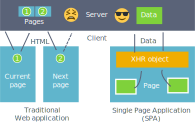
\includegraphics[width=1.0\linewidth]{assets/img/spa-bis.pdf}
	\caption{Difference between traditional Web applications and Single Page Application (SPA). A traditional application will ask the server to generate a new HTML page to access the required content. A SPA will just ask for the required data and render it in the client directly.}%
	\label{fig:spa}
\end{figure}

\subsubsection{Angular}%
\label{ssub:angular}

AngularJS~\cite{hevery2009declarative} goes back to 2009, when Miško Hevery and Adam Abrons
where trying to sell online storage services through software at getangular.com.
The project wasn't successful enough, and so they made <angular/> open source.
Miško Hevery was later recruited at Google, working on their feedback project.
The story, as told by Miško Hevery and Brad Green at Google I/O 2013~\cite{angularjs-googleio},
says that it took Miško three weeks (though he had bet two) to rewrite a six-month work
with 17000 lines of code into 1500 lines of code with <angular/>.
Impressed, Brad decided to embrace the <angular/> project under Google's wing
and it got rebranded AngularJS with a new logo.
In 2016, Google released its successor, renamed Angular (without the JS part).
An important difference is that Angular is using TypeScript instead of JavaScript.
The key feature of Angular/AngularJS is declarative two-way data binding,
showcased in Listing~\ref{lst:angularjs}.
Another important design decision is that Angular is trying
to provide a fully featured and coherant framework
capable of handling most use cases you will ever encounter.

\lstinputlisting[%
  language=HTML,
  caption={Two-way data binding in AngularJS.},
  label={lst:angularjs}
]{assets/code/angularjs.html}

\subsubsection{React}%
\label{ssub:react}

Contrary to Angular, React is designed to solve a very specific use case,
which is how to build user interfaces.
As such it doesn't care about how you store data,
or manage routing of the SPA with the url.
The core feature of React is its Virtual DOM that we will explain soon.
It provides one-way data binding between the state of a React component
and its rendering in the DOM.\@
The syntax used for the binding is showcased in Listing~\ref{lst:reactjs}.

\lstinputlisting[%
  language=ES6,
  caption={React example showing the state and render function of a component.},
  label={lst:reactjs}
]{assets/code/react.js}


\subsubsection{Vue}%
\label{ssub:vue}

Vue describes itself as a progressive framework,
meaning it provides core features targetting a small scope,
and other opt-in layers bringing more functionalities.
In a sense, it shares advantages and inconvenients of both
React and Angular, with a different balance point.
It mostly uses one-way data bindings,
but also provides inbuilt conveniences to simulate two-way data binding
through attaching event listeners when using the ``v-model'' property.
An example is given in Listing~\ref{lst:vuejs}.

\lstinputlisting[%
  language=HTML,
  caption={Simulated two-way data binding in Vue using the ``v-model'' property.},
  label={lst:vuejs}
]{assets/code/vue.html}


\subsection{Functional reactive programming}%
\label{sub:functional_reactive_programming}

Elm, FRP research papers.

\subsection{Virtual DOM}%
\label{sub:virtual_dom}

Why modifying the DOM directly is a mistake.
Understanding the animation frame loop.

\subsection{Assets compilation}%
\label{sub:assets_compilation}

How JavaScript switched from a human readable interpreted file,
to a modularized, transpiled, minified, gzipped compilation target.


\subsection{How to choose?}%
\label{sub:how_to_choose_}

All three frameworks provide data binding between the state of the application
and its rendering, making the user interface declarative and reactive.
Angular and React are the more mature projects with
the biggest community.
Angular provides a solution covering most aspects needed for a SPA,
while React is focused on the user interface and will often be paired
with libraries to manage state efficiently like Redux.
Vue has a lower barrier to entry, like React,
but also a coherent set of opt-in functionalities making it an all-in-one solution similar to Angular.
In order to produce small and compatible applications,
they all require multiple techniques such as modularization,
transpilation or minification, effectively making Web development similar
to static and compiled development environments.
Knowing all this, I will argue that we can use Elm,
a functional programming language compiling to JavaScript.
In the next section I will detail how it can bring
all the advantages of other Web frameworks,
but with an improved developer experience,
and a more reliable application at the end.

\section{Elm}%
\label{sec:elm}

Elm is a statically typed functional programming language for building Web applications.
Its syntax comes from the ML family of languages, similar to Haskell and OCaml.
The home page of the language claims that Elm generates JavaScript
with great performances and no runtime exceptions.
In the following sections, we will see how its properties enable such a claim.

\subsection{Pure functions}%
\label{sub:pure_functions}

All functions in Elm, except for debugging, are ``pure'',
meaning they produce no side effect.
A side effect is a behavior with implications outside of the scope of a function,
such as modifying a global variable or an input parameter,
generating random values or interacting with the outside world.
Side effects are important to handle to build applications that are not predetermined
at startup, but we will explain later how they are managed withing The Elm Architecture (TEA).

Listing~\ref{lst:sideeffectjs} gives examples of functions that cannot be directly
transcribed from JavaScript to Elm due to side effects.
Pure functions are also sometimes called ``referentially transparent''
though the meaning of this terminology is unclear depending on sources.
The important property is that calling a pure function with the same arguments
will always return the same result.
As a consequence many optimizations can be performed such as memoization,
or precomputation of functions with no arguments (which actually are constant expressions).
The Elm compiler doesn't precompute constant expressions yet,
but memoization in the form of lazy functions can be used for computation
of view functions, reducing the amount of work for the diffing algorithm
of the virtual DOM.\@

\lstinputlisting[%
  language=ES6,
  caption={Side effects in JavaScript.},
  label={lst:sideeffectjs}
]{assets/code/side-effect.js}


\subsection{Algebraic Data Types (ADT)}%
\label{sub:algebraic_data_types_adt_}

Algebraic data types (ADT) initially appeared in 1980 with the Hope programming language,
developed by Rod Burstall, Dave MacQueen and Don Sannella~\cite{burstall1980hope}.
Since then, they have been popularized by functional programming languages
such as Haskell or OCaml.
Usually, algebraic data types include product types and sum types.
Product types are types regrouping multiple data together under the same name.
Tuples like (Int, Float), and records (or objects) are the most common product types.
Their names come from the properties on cardinality if we consider types as sets.
Indeed, a tuple of three booleans have a cardinality of 8 if you consider
all possible combinations, which is the product $2\times2\times2$.
Sum types are referred to as ``custom types'' in Elm.
They are defined with the ``type'' keyword.
Few examples of custom types definitions are provided in Listing~\ref{lst:customtype-elm}.
\comment{}{OneOfThreeBools as 6 distinct elements, 2 + 2 + 2}

\lstinputlisting[%
  language=Elm,
  caption={Custom types definitions in Elm.},
  label={lst:customtype-elm}
]{assets/code/customtype.elm}

The most important property of custom types in Elm
is that they enable modelization of a problem with exactly the correct
cardinality for the types, preventing impossible states by design.
Concretely, consider that we are modeling accessibility of a site
depending on the logged status of users.
Typically, in a language without sum types, like JavaScript,
the user will be modeled with two fields as in Listing~\ref{lst:userjs}.
Initially the ``loggedIn'' field will be false and the user name empty.
And as soon as the user is logged in,
the corresponding field will have the value ``true'',
and the name will be filled with the user name.
But what happens when the ``loggedIn'' field is ``false'' but
the name is filled with something like ``John Doe''.
In theory this state should never be reached if we are carefull in our implementation,
but in practice, bugs tend to fill every possible crack,
requiring more tests to verify that this state is never reached.
With custom types in Elm, the user type will be defined as in Listing~\ref{lst:userelm}.
In this definition, a user can either be anonymous or logged in with a name,
but never anonymous and with a name.
By design, custom types prevents an entire family of bugs.

\lstinputlisting[%
  language=ES6,
  caption={User modeled with a product type in JavaScript.},
  label={lst:userjs}
]{assets/code/user.js}

\lstinputlisting[%
  language=Elm,
  caption={User modeled with a custom (sum) type in Elm.},
  label={lst:userelm}
]{assets/code/user.elm}


\subsection{Total functions}%
\label{sub:total_functions}

Functions are qualified as ``total'' when they are guarantied
to return a result for every possible valid input.
\comment{}{Actually find a precise definition here.}
\comment{}{Advantages of total functions.}
Elm has two properties helping in the quest of total functions,
\begin{itemize}
	\item exhaustive pattern matching on custom types,
	\item and no statement, only expressions.
\end{itemize}

\subsubsection{No statement, only expressions}%
\label{ssub:no_statement_only_expressions}

In most programming languages like JavaScript,
programs are composed of successions of statements and expressions.
The former do not return values while the latter do.
Appart from imports, Elm code contains only top level definitions and expressions.
Listing~\ref{lst:expressionelm} provides example of Elm expressions
for conditions or loops.
All branches of conditions (``if'' expressions) must have a value of the same type.
Without an ``else'' branch, the code will not compile.
Not having ``for'' loops statements is among the thoughest functional
concepts to learn for begginers.
In a language with only expressions,
loops need to be expressed either with recursive functions,
or with higher order functions, like ``List.foldl'' in the length example.

\lstinputlisting[%
  language=Elm,
  caption={Branching control and loops are expressions in Elm.},
  label={lst:expressionelm}
]{assets/code/expression.elm}


\subsubsection{Pattern matching}%
\label{ssub:pattern_matching}

Pattern matching is a branching mechanism based on the structure of a type.
Any custom type can be matched to one of its different variants
with the ``case ... of'' syntax as shown in Listing~\ref{lst:pattern-matching-elm}.
Any lowercase variable in the pattern will be bound to the corresponding data,
like the ``name'' variable here.

\lstinputlisting[%
  language=Elm,
  caption={Pattern matching in Elm},
  label={lst:pattern-matching-elm}
]{assets/code/pattern-match.elm}

In javascript, one can fairly easily forget to handle a case,
or willingly only process the ``happy path'' for prototyping speed.
In Elm, if I remove the ``Anonymous'' branch,
the compiler will refuse to compile the code
with the message showed in Listing~\ref{lst:missing-pattern-elm}

\lstinputlisting[%
  language=Elm,
  caption={Missing pattern compiler error in Elm},
  label={lst:missing-pattern-elm}
]{assets/code/pattern-match-missing.elm}

As suggested in the hint of the compiler error,
we can also use the ``Debug.todo "message"'',
which is very useful for the rapid prototyping phase.
Remark that the ``Debug.todo'' function will make the program crash
if reached at runtime.
For this reason, all functions from the ``Debug'' module
are forbidden in code compiled in release mode.


\subsubsection{No runtime exception}%
\label{ssub:no_runtime_exception}

Thanks to expressions and exhaustive pattern matching,
Refactoring an Elm code base can be done with confidence.
Any place where types do not match with functions
will be signalled by the compiler, which becomes a true coding assistant.
Noredink, a company based in San Francisco reported in 2018 that after
two years of using Elm in production,
they got their first runtime exception,
compared to 60000 for the JavaScript code~\cite{zeroruntimeerror}.


\subsection{The Elm Architecture (TEA)}%
\label{sub:the_elm_architecture_tea_}

\begin{figure}[ht]
\includegraphics[width=\columnwidth]{assets/img/tea-draw-io.pdf}
\caption{The Elm Architecture (TEA).}%
\label{fig:tea}
\end{figure}

The Elm Architecture (TEA) enforces a unidirectional data transformation flow,
visualized in Figure~\ref{fig:tea}.
The central entity is the \verb|Model|.
It contains all and every information about our application state.
The visual aspect of our application is called the \verb|View|
(basically an HTML rendered document) which is generated by the \verb|view| function,
from the \verb|Model|. Finally, all events generate messages, of type \verb|Msg|.
The \verb|update| function, updates the model by reacting to those messages, closing the loop.

All functions are pure, meaning there is no side effect,
outputs of functions are entirely defined by inputs.
There cannot be global variables mutations,
real world events, network interaction etc.
Basically such a program would be running in a predestined way
from its start to its end,
preventing us from loading images and interacting with them.
This is why the application is attached to the Elm runtime,
provided by the language, transforming all real world events (``side effects'')
into our defined set of messages, of type \verb|Msg|.

The main challenge with pure functions is
to describe side effects without performing them.
Those are described in three locations:

\begin{enumerate}
\item View attributes as DOM event listeners for pointer events.
\item Commands (\verb|Cmd|) generated by the update function, like loading of images.
\item Subscriptions (\verb|Sub|) to outside world events like the window resizing.
\end{enumerate}

The Elm runtime takes those side effect descriptions,
perform them, and, whenever there is a result / an answer,
transforms it into one of our defined messages (\verb|Msg|)
and routes it to our update function.
After updating the model, the runtime automatically calls the \verb|view| function.
This way, the user interface reacts to model modifications
similarly than with other one-way data bindings we have previously introduced.


\subsection{Elm-UI, an alternative layout strategy}%
\label{sub:elm_ui_an_alternative_layout_strategy}

\begin{figure}[ht]
	\centering
	\setlength{\fboxsep}{0pt}
	\fbox{\includegraphics[width=1.0\linewidth]{assets/img/elm-ui.png}}
	\caption{User interface specified by Listing~\ref{lst:elm-ui}.}%
	\label{fig:elm-ui}
\end{figure}

We have seen that the Elm architecture enables building Web applications with HTML views.
It treats the user interface as data, using a virtual DOM under the hood
and managing the DOM side effects with a runtime system.
Overall, with Elm guaranties, one is fairly confident that when
the program compiles, it is functionally correct.
Layout however, traditionally relies both on HTML and CSS rules,
intrinsically hard to debug due to their cascading nature
since a CSS rule may apply to all children of a DOM element.
In~\cite{sinha2015simplifying}, Sinha et al. identified user interface design
as the main difficulty in Web development.

At Elm Europe 2017, Matthew Griffith made a presentation
entitled ``Understanding style''~\cite{griffithstyle}.
In this work, he identifies the most problematic aspect of layout being
that there is no clear way to identify when it is incorrect.
There is not even an unhelpful ``undefined is not a function'' in CSS resolution.
Basically an error in layout and style is just the unexpected.
With this in mind he created library, now named elm-ui~\cite{griffithelmui},
aiming at providing the guaranty that if your code compiles,
the layout if fully specified.
They key property of the library is that its base building block,
the ``el'' element only has one child,
instead of a list like in the case of a ``div'' HTML element.
Also, building blocks with multiple children must have explicit layout.
Listing~\ref{lst:elm-ui} showcases how functional composition of UI elements
and an attention on naming enable building of clear and robust user interfaces.
The corresponding user interface is provided in Figure~\ref{fig:elm-ui}.

\lstinputlisting[%
  language=Elm,
  caption={Fully specified layout with elm-ui.},
  label={lst:elm-ui},
  basicstyle=\scriptsize\ttfamily
]{assets/code/elm-ui.elm}

\chapter{Interactive Annotation on the Web}%
\label{cha:interactive_annotation_on_the_web}

\lstset{language=haskell, style=CodeStyle}

\section{Introduction}

\begin{figure}[ht]
  \includegraphics[width=\textwidth]{assets/img/annotation-app-thin.jpg}
  \caption{Screenshot of the interface of our image annotation Web application.}%
  \label{fig:teaser}
\end{figure}

Image annotations are required in a wide range of applications
including image classification (which requires textual labels),
object detection (bounding boxes), or image segmentation (pixel-wise classification).
The rise and successes of deep learning lead to an increasing need for annotations,
as training sets should be of a large size for these algorithms to be efficient.
Yet, researchers still spend time and resources
to create ad hoc tools to prepare those datasets.
The application we present in this paper aims at providing a customizable tool
to fulfill most image annotation needs.

\begin{table*}[ht]

\begin{tabular}{lclllcc}
Application
	& Year
    & Tools
    & \makecell[l]{Configurable\\interface}
    & \makecell[l]{Tasks\\management}
    & Type
    & License \\
    \midrule
LabelMe
	& 2008
    & bbox, polygon, iterative semi-automatic segmentation
    & no
    & Mturk integration
    & server
    & OSS \\
VIA
	& 2016
    & bbox, polygon, point, circle, ellipse
    & no
    & no
    & client
    & OSS \\
Labelbox
	& 2018
    & bbox, polygon, point, line
    & yes
    & yes
    & server
    & private \\
Dataturks
	& 2018
    & bbox, polygon
    & no
    & yes
    & server
    & private \\
Ours
	& 2018
    & bbox, polygon, point, stroke, outline
    & yes
    & Mturk integration
    & client
    & OSS \\
\end{tabular}

\caption{Most relevant image annotation Web applications.}%
\label{tab:web-apps}
\end{table*}

% \begin{figure*}[ht]
%     \centering
%     \begin{subfigure}[b]{0.575\textwidth}
%         \includegraphics[width=\textwidth]{assets/img/labelme.jpg}
%         \caption{LabelMe}
%     \end{subfigure}
%     \hfill
%     \begin{subfigure}[b]{0.405\textwidth}
%         \includegraphics[width=\textwidth]{assets/img/via.jpg}
%         \caption{VIA}
%     \end{subfigure}
%     \hfill
%     \begin{subfigure}[b]{0.42\textwidth}
%         \includegraphics[width=\textwidth]{assets/img/dataturks.jpg}
%         \caption{Dataturks}
%     \end{subfigure}
%     \hfill
%     \begin{subfigure}[b]{0.56\textwidth}
%         \includegraphics[width=\textwidth]{assets/img/label-box-config.jpg}
%         \caption{Labelbox}
%     \end{subfigure}
%     \caption{Interfaces of main other Web annotation applications}\label{fig:interfaces}
% \end{figure*}

Many image annotation applications already exist (Table~\ref{tab:web-apps}).
LabelMe~\cite{russell2008labelme}, one of the most popular,
provides an interface for drawing bounding boxes and polygons
around objects in an image.
It has been used extensively to create datasets for image segmentation.
Some more recent softwares share the same goals, with their own specificities.
For example, Labelbox~\cite{labelbox} and
Dataturks~\cite{dataturks} provide annotation tasks management,
particularly useful when crowdsourcing the annotations;
these softwares are proprietary.
The VGG Image Annotator (VIA~\cite{dutta2016via})
is an open-source client application like ours,
with the specificity of providing annotation attributes,
editable in a spreadsheet format.

We release an open-source application~\cite{annotationappgithub},
entirely client side, meaning that no data is uploaded to any server.
Images are loaded from files and annotated locally, in the browser.
The simplest tool, from a user perspective, should be immediately available
i.e.\ should not require any additional installation to be fully functional.
Our image annotation software is thus a Web-based application,
easily configurable to fit users needs, as well as
embeddable in the Mechanical Turk platform to design crowdsourcing campaigns.

We first present the features of our application, then describe its architecture.
Finally, we explain how it can be used to start crowdsourcing experiments.


\section{Presentation of the application}

A screenshot of the application can be seen in Figure~\ref{fig:teaser}.
The image to be annotated occupies the central part of the screen;
a toolbar is located on top, object classes are available on the left
and images to be annotated on the right.


\textbf{Images}.
Multiple images can be loaded at the same time using the image icon
on the top-right corner of the application.
These images are not uploaded on the server,
and can either be loaded locally from the client's machine,
or from a distant server.
% * <matthieu.pizenberg@gmail.com> 2018-05-20T06:53:31.040Z:
% 
% > or from a distant server.
% Seulement quand c'est fait directement dans le champ images des "flags" au démarrage de l'appli, pas en cliquant sur le bouton
% 
% ^ <matthieu.pizenberg@gmail.com> 2018-05-20T09:57:23.955Z.


\textbf{Tools}.
Our application includes several tools to annotate images.
Icons for these tools are depicted in Figure~\ref{fig:icons}.
From left to right, the first available annotation is the point,
that can be useful to designate objects in the image.
It can also be used as a seed in region-growing image segmentation methods.
The second annotation we included is the bounding box,
which provides the localization of objects in the image,
and is used in object detection problems.
The information we acquire are the left, right, top and bottom coordinates
of the bounding box.
The third annotation we chose to implement is the stroke,
or scribble, which is a popular interaction in image segmentation.
It consists in a sequence of points, interpreted as a continuous line.
The outline, fourth type of annotation,
is a closed shape, typically drawn around objects.
It is comparable to a bounding box in essence,
but provides a more precise location of objects.
Finally, polygons can also be drawn (as in LabelMe, for instance),
by successively clicking new points as vertices.


All these tools are available both with a mouse or a touch interaction.
As a matter of fact, some tools are better suited to touch devices
(for example, outlines) than others (polygons).

\begin{figure}[ht]
\centering
\includegraphics[width=0.8\columnwidth]{assets/img/annotation-tools.png}
\caption{Annotation tools icons}%
\label{fig:icons}
\end{figure}


\textbf{Object classes}.
For most annotation tasks, we also need to differentiate objects in the images.
Typically each annotated area is attributed a class, or label.
The PASCAL VOC dataset~\cite{everingham2010pascal}, for example,
is composed of 20 classes, grouped by categories:
\begin{itemize}
\item \textit{Person}: person
\item \textit{Animal}: bird, cat, cow, dog, horse, sheep
\item \textit{Vehicle}: aeroplane, bicycle, boat, bus, car, motorbike, train
\item \textit{Indoor}: bottle, chair, dining table, potted plant, sofa, tv/monitor
\end{itemize}

In our application, classes are specified in a JSON configuration file.
A strict corresponding config for PASCAL VOC classes
is presented in Listing~\ref{lst:pascal}.

\lstinputlisting[language=json,caption={A configuration file to annotate the PASCAL dataset.},float,label={lst:pascal}]{assets/code/config-pascal.json}

To attribute a class to an annotation,
a user should first select the class in the left sidebar,
then use a tool to create an annotation.
Selecting a class in the left sidebar also highlights the annotations
corresponding to this class.


\textbf{Configuration file}.
The five annotation tools are optionally made available by the configuration file.
In Listing~\ref{lst:pascal}, the last line of the depicted configuration file
contains an \texttt{annotations} field, listing the tools that should be available.
In this case, they all are.

In addition to the five fundamental annotation types,
each type can be derived in virtually any number of variations.
For example, interactive segmentation algorithms often require
\textit{foreground} and \textit{background} scribbles.
In our application, this would mean the user would need to draw two types of strokes.
This can be achieved using the configuration file,
as in Listing~\ref{lst:variations}.
Such configuration would result in two stroke icons in the toolbar,
of different colors, just as in Figure~\ref{fig:teaser}.

\lstinputlisting[language=json,caption={A configuration file to include two types of strokes.},float,label={lst:variations}]{assets/code/config-variations.json}


\section{Technical choices}

The application code is organized in two parts:

\begin{itemize}
\item A minimalist Node.js server, located in the \verb|server/| directory.
	It is statically serving the content of \verb|server/dist/|
    with compression.
\item A complete Elm client application, located in the \verb|client/| directory.
    Elm~\cite{czaplicki2013asynchronous,czaplicki2017elm}
    isn't a JavaScript framework, it is a functional programming language,
	compiling to JavaScript to run in browsers.
	Its syntax is inherited from Haskell but far simpler.
	The compiled application is 150 KB gzipped,
    which is great for low bandwidth connections.
\end{itemize}


\subsection{The application architecture}

\begin{figure}[ht]
\includegraphics[width=\columnwidth]{assets/img/tea-draw-io.pdf}
\caption{The application architecture.}%
\label{fig:tea}
\end{figure}

The application architecture enforces a unidirectional data transformation flow,
visualized in Figure~\ref{fig:tea}.
The central entity is the \verb|Model|.
It contains all and every information about our application state.
The visual aspect of our application is called the \verb|View|
(basically an HTML rendered document) which is generated by the \verb|view| function,
from the \verb|Model|. Finally, all events generate messages, of type \verb|Msg|.
The \verb|update| function, updates the model by reacting to those messages, closing the loop.

All functions are pure, meaning there is no side effect,
outputs of functions are entirely defined by inputs.
There cannot be global variables mutations,
real world events, network interaction etc.
Basically such a program would be running in a predestined way
from its start to its end,
preventing us from loading images and interacting with them.
This is why the application is attached to the Elm runtime,
provided by the language, transforming all real world events (``side effects'')
into our defined set of messages, of type \verb|Msg|.

The main challenge with pure functions is
to describe side effects without performing them.
Those are described in three locations:

\begin{enumerate}
\item View attributes as DOM event listeners for pointer events.
\item Commands (\verb|Cmd|) generated by the update function, like loading of images.
\item Subscriptions (\verb|Sub|) to outside world events like the window resizing.
\end{enumerate}

The Elm runtime takes those side effect descriptions,
perform them, and, whenever there is a result / an answer,
transforms it into one of our defined messages (\verb|Msg|)
and routes it to our update function.


\subsection{The model states}

The \verb|state| is the main component of the \verb|Model|.
It contains the images and configuration loaded as well as the annotations performed.
Its type is defined as in Listing~\ref{lst:state}
and can be modeled as a finite state machine, visualized in Figure~\ref{fig:states}.

\lstinputlisting[language=elm,caption={State type definition.},label={lst:state},float]{assets/code/State.elm}

\begin{figure}[ht]
\centering
\includegraphics[width=\columnwidth]{assets/img/states-draw-io.pdf}
\caption{The application states.}%
\label{fig:states}
\end{figure}

The application available online starts in state 0 (\verb|NothingProvided|)
and enables you to reach state 2 (\verb|AllProvided|)
with buttons to load images and configuration.
Two messages called \verb|LoadImages| and \verb|ConfigLoaded| produce
transitions in the state machine.


\subsection{The messages}

All modifications of the model are understood
by looking at the \verb|Msg| type definition (Listing~\ref{lst:msg}).
The \verb|update| function then performs the modifications described by those messages.

\lstinputlisting[language=elm,caption={Msg type definition.},label={lst:msg},float]{assets/code/Msg.elm}

\begin{itemize}
\item The \verb|WindowResizes| message is triggered when the application is resized.
	In the update function, it takes the new size and recomputes some view parameters.
\item A \verb|PointerMsg| message is triggered by pointer events (mouse, touch, etc.).
	In the update function, this is the message activating
	all the annotations logic code of our application.
\item The messages \verb|SelectImage|, \verb|SelectTool| and \verb|SelectClass|
	are generated when clicking on images, tools and classes.
\item Files are handled by five messages:
	\begin{itemize}
	\item When loading images from the file explorer,
		a \verb|LoadImages| message is generated with a list of the images files
		and their names as identifiers.
		For each image correctly loaded an \verb|ImageLoaded| message is generated,
		providing a local url, corresponding to the image in memory.
    \item The messages \verb|LoadConfig| and \verb|ConfigLoaded| behave similarly.
    \item The \verb|Export| message causes the application to serialize into JSON
		all the annotations, and asks the user to save the generated file.
		It is triggered by clicking on the export button of the top action bar.
	\end{itemize}
\item Whenever an event should change the zooming level of the drawing area,
	a \verb|ZoomMsg| message is  generated.
\item Finally, the \verb|RemoveLatestAnnotation| message is also explicit.
\end{itemize}


\subsection{The view}

The view of this application is based on four components,
each implemented in its own module, with potentially different versions
depending on the current state of the application.
\begin{itemize}
\item The top action bar (\verb|src/View/ActionBar.elm|).
\item The center annotations viewer area\\(\verb|src/View/AnnotationsArea.elm|).
\item The right images sidebar\\(\verb|src/View/DatasetSideBar.elm|).
\item The left classes sidebar\\(\verb|src/View/ClassesSideBar.elm|).
\end{itemize}


% \subsection{Startup and interactions with JavaScript}

% Compiling the Elm application code produces a JavaScript file \verb|Main.js|.
% This file has to be embeded in an html document.
% Then the application is started with parameters called "flags"
% as demonstrated in Listing~\ref{lst:start}.

% \lstinputlisting[language=javascript,caption={JavaScript code to embed the Elm application.},label={lst:start},float]{assets/code/start.js}


\subsection{Library and application duality}

In order to offer a turnkey solution to image annotations,
we created a configurable application solving most needs.
But we also thought of cases where advanced modifications are required.
Consequently, the foundation of this application has been extracted
in the independent package elm-image-annotation~\cite{annotationpackage}.
It is designed as an API to create, modify and visualize geometric shapes,
useful in the context of image annotation.

Modules for manipulation and serialization (in JSON) of annotations are
under the \verb|Annotation.Geometry| namespace.
It already contains one module for each tool presented earlier.
If you want to introduce a new tool, this is where you can create a new module.

This package also contains the following important modules,
under the \verb|Annotation| namespace:
\begin{itemize}
	\item \verb|Annotation.Style|:
		defines types describing appearance of points, lines and fillings of annotations.
	\item \verb|Annotation.Svg|:
		exposes functions rendering SVG elements for each annotation kind.
	\item \verb|Annotation.Viewer|:
		manages the central visualization area,
		supporting zooming and translations, relative to an image frame.
\end{itemize}
If you are interested in creating another rendering target than SVG,
like canvas, WebGL, \ldots, it would require alternative modules
to \verb|Annotation.Svg| and \verb|Annotation.Viewer|.
The rest of the code can stay unchanged.


\section{Crowdsourcing annotations}

Image annotation interfaces are often used in the context
of large datasets of images to annotate.
As such, tasks management for crowdsourcing campaigns is an important feature. 
Labelbox and Dataturks are all-in-one services providing
tasks management directly in their applications.
Just like LabelMe, we choose instead to provide a configuration,
ready to use with Amazon Mechanical Turk (Mturk).

Mturk comes in two sides. A ``requester'' is defining a set of tasks
while a ``worker'' is performing them.
Workers are payed by requesters through Mturk service.
The concept of a ``HIT'' (Human Intelligence Task) characterizes the task unit.
In our case, one HIT means one image to be annotated.
We describe in details how to setup a campaign with our template
in the application documentation.


\section{Conclusion}

In this paper we have introduced our web-based image annotation application.
More information is available in the online documentation~\cite{annotationappdoc}.
The application is still actively developed, we welcome all feedback and contributions.


\section{Acknowledgments}

We would like to thank:

\begin{itemize}
	\item @tforgione and @GarciaDelMolino for your wise feedbacks.
	\item @dncg for your Windows tests.
	\item The online Elm community for their help along the road:
		@evancz for the delightful Elm language,
		@ianmackenzie for your fantastic geometry library,
		@mdgriffith for your very refreshing layout library,
		@luke for the amazing tool Ellie,
		@norpan, @jessta, @loganmac, @antew, for your invaluable help on slack.
\end{itemize}



\part{RGB-D SLAM}%
\label{prt:rgb_d_slam}
This part is about RGB-D SLAM\@.

\chapter{The RGB-D SLAM Problem}%
\label{cha:the_rgb_d_slam_problem}

Introduce RGB-D SLAM algorithms.

\begin{itemize}
	\item Image formation
	\item Multiple view geometry
	\item Structure from motion
	\item Visual SLAM
	\begin{itemize}
		\item Visual odometry (mention RGB-D here?)
		\item Pose graph
		\item Loop closure
	\end{itemize}
	\item Direct VS indirect methods
	\begin{itemize}
		\item Feature points (sift, fast, orb, ...)
		\item Direct formulation
	\end{itemize}
\end{itemize}

\chapter{Contribution on RGB-D Visual Odometry}%
\label{cha:contribution_on_rgb_d_visual_odometry}

Explain vors (pas encore publié).

\begin{itemize}
	\item RGB-D Tracking Evaluation
	\item Visual Odometry in Rust (vors)
	\begin{itemize}
		\item Candidate points selection (coarse to fine)
		\item Multi-resolution image gradients
		\item Multi-resolution direct image alignment
		\item Levenberg-Marquardt (non-linear optimization)
		\item Gradients of the reprojection function (inverse compositional)
		\item Robust optimization techniques
		\item Photometric term in the residuals
	\end{itemize}
\end{itemize}

\chapter{Performant Web Applications}%
\label{cha:performant_web_applications}

History of native code on the Web: Java, Flash, nacl, etc.

\begin{itemize}
	\item WebAssembly
	\begin{itemize}
		\item Minimum Viable Product (MVP)
		\item Bright future: wasi, wapm, ...
	\end{itemize}
	\item History of Emscripten
	\begin{itemize}
		\item LLVM
		\item asmJS
		\item wasm
	\end{itemize}
	\item C++ portability pitfalls
	\item Rust to wasm (wasm-bindgen)
	\begin{itemize}
		\item Rust programming language
		\item Wasm-bindgen
	\end{itemize}
\end{itemize}

\chapter{Interactive SLAM on the Web}%
\label{cha:interactive_slam_on_the_web}

Find something to do XD\@.


\chapter*{Conclusion}%
\label{cha:conclusion}
\addcontentsline{toc}{chapter}{Conclusion}
At the beginning of this journey, we asked ourselves
how user interactions and the Web can improve computer vision research.
Throughout this work, we showcased different approaches to combine those capabilities
within interactive computer vision Web applications.

In the case of image annotation, we provided an adaptation of the GrabCut algorithm
combined with medial axis transforms to retrieve precise segmentations from outlining.
This interaction has been integrated into a reliable Web application
to crowdsource segmentation annotations of the PASCAL-VOC dataset.
The clear benefit illustrated here is the scaling and the reach that the Web
offers for the creation of learning datasets.

Visual odometry is a computationally intensive task.
Due to previous limitations of the Web platform, running those applications directly
in a browser was not sufficiently efficient to be seriously considered.
The advent of new technologies such as WebAssembly, or WebGL changed this vision completely.
Therefore, we started a new visual odometry library in a recent programming
language named Rust with excellent support of WebAssembly.
We showed how this library can be integrated in a Web application,
and profit from its interactive nature to improve the tracking results.
This example paves the way for easy access to computer vision algorithms,
both for research reproducibility and availability to a non technical public
such as creators.

We described how image segmentation and visual odometry can take advantage
of user interactions when made accessible through the Web.
To this end, we provided concrete explanations on how to build reliable Web applications,
and how to port computationally intensive tasks to run the browser.
Generally, this approach has the potential to improve machine learning
and other computer vision fields thanks to exposure to a wider,
more varied set of data.
Yet I don't see this practice being picked up immediately.
In fact, mainstream solutions for computer vision have a strong inertia
due to the massive amount of already available libraries in C++ and Python.
It will thus take time before performant languages better suited for the Web like Rust
obtain fair usage share and push more research to public exposure through the Web.
Our specific contribution in image segmentation also have limitations.
The segmentations obtained with single outlines for example do not always
provide perfect masks. One could then reasonably question the viability of that interaction
to create learning datasets.

Future work could address that point about the loss of precision when using outlines
or other imperfect interactive segmentation methods.
The aim would be to find a balance point between annotation speed and prediction quality.
In particular, we would like to study how loss in precision for the training data translates
into loss of quality for machine learning algorithms,
and how regularization techniques can minimize the effect of noisy training data.
Regarding the visual odometry library, there are many improvements that we could work on,
both on the research and the platform sides.
One future goal is to be able to run reliably and smoothly on mobile devices.
Smartphones typically run on ARM processors, a target supported natively
by the Rust toolchain, and also through WebAssembly runtimes so there should not be
huge platform hurdles.
They are often equiped with more sensors that dedicated cameras
such as inertial measurement units (IMU).
Integrated smartphones cameras however, usually feature rolling shutter sensors,
which change the image formation modelization.
Among the many possible research extensions, the priorities are
the adaptation to the RGB case (no depth),
photometric variation modelization to account for automatic exposure,
modelization of rolling shutter and fusion with IMU data.
Another very exciting avenue to explore could be collaborative
SLAM through the Web.
Since smartphones are now connected to high speed 4G and 5G networks,
we could imagine situations where groups of individuals all take part
in one global map optimization process.

These are exciting times to be alive!
Admittedly, we will not radically change every aspect of our lives
with better segmentation maps or increased visual odometry precision.
But as we mentioned in the introduction, those are key aspects
of technological evolutions that could impact our society such as autonomous vehicles.
From 1830 to 1890 the distance of railroad in operation in the United States
grew from 23 to 166706 miles~\cite{depew1895one}.
With that growth, the number of brakemen deaths (cf Figure~\ref{fig:brakeman}) also radically
increased until the introduction of air brakes which replaced their jobs by safer systems.
It is a matter of time, continued research and social acquaintance,
but autonomous vehicles will eventually provide a similar transformation
from manual to automatic systems; and
I hope this work will be a positive contribution to a better future.


\begin{figure}[b]
	\centering
	\includegraphics[width=0.5\textwidth]{assets/img/brakeman-peckwell-apicnic.jpg}
	\caption{Representation of brakemen, who used to work in all weather conditions.
	``A Picnic'', engraving by Peckwell, published on the cover of The Railroad Conductor, vol. 7, no. 15 (Aug. 1, 1890).
	Image in public domain.}%
	\label{fig:brakeman}
\end{figure}

% \begin{figure}[b]
% 	\centering
% 	\includegraphics[width=0.5\textwidth]{assets/img/easymile-bus.jpg}
% 	\caption{Easymile autonomous bus in Bad Birnbach.
% 	Published under Creative Commons by Rudolf Simon, January 2018.}%
% 	\label{fig:easymile}
% \end{figure}


% Back matter #######################################################
\backmatter%

\bibliographystyle{plain}
\bibliography{%
	src/mainmatter/annotation/interactions.bib,
	src/mainmatter/annotation/outlining.bib,
	src/mainmatter/annotation/web.bib
}
